% =====================================================================================
% 0_main.tex: the paper's root document: packages, commands, sections.
%
% Build (from paper/):
%   tectonic -X compile 0_main.tex          # or: latexmk -pdf 0_main.tex
% Sections are numbered files (0_abstract.tex, 1_introduction.tex, ..., 4_experiments.tex); a
% missing one is skipped, so the document builds while the paper is being written.
% Tables are table_<name>.tex next to this file, figures figures/fig_<name>.tex.
%
% TODO(venue): replace the document class / style file by the venue's template; the
%   commands below are independent of it.
% =====================================================================================
\documentclass[10pt]{article}

% ---- packages ------------------------------------------------------------------------
\usepackage[utf8]{inputenc}
\usepackage[T1]{fontenc}
\usepackage{lmodern}
\usepackage[margin=2.2cm]{geometry}
\usepackage{amsmath,amssymb}
\usepackage{graphicx}
\usepackage{booktabs}
\usepackage{multirow}
\usepackage[table]{xcolor}
\usepackage{microtype}
\usepackage[hidelinks]{hyperref}
\usepackage[capitalise,noabbrev]{cleveref}   % after hyperref

% ---- names -----------------------------------------------------------------------------
% Every model / method name of the paper goes through one of these commands: change a
% name here and it changes in the text, the tables and the figure captions. Use them with
% {} (\ours{}) so the following space is kept.
\newcommand{\logix}{LogiX-GIN}                  % upstream method (NeurIPS 2025)
\newcommand{\ours}{Proto-LogiX-GIN}             % TODO(name): our method, name not decided
\newcommand{\nmp}{NMP}                          % node prototypes with care mask and push
\newcommand{\qat}{QAT}                          % quantisation-aware fine-tune
\newcommand{\nmpqat}{\nmp{}+\qat{}}
\newcommand{\teacher}{GIN teacher}

% Rows of the tables (one command per model)
\newcommand{\classic}{\logix{} (mean, max, sum)}  % upstream readout
\newcommand{\classicnosum}{\logix{} (mean, max)}  % without sum pooling
\newcommand{\oursgraph}{\ours{} (graph)}          % graph-level prototypes
\newcommand{\oursnmp}{\ours{} (\nmp{})}           % node prototypes
\newcommand{\oursqat}{\ours{} (\nmpqat{})}        % node prototypes + QAT (rule model)

% ---- table cells -------------------------------------------------------------------------
\newcommand{\ms}[2]{$#1{\scriptstyle\,\pm\,#2}$}  % mean ± std
\newcommand{\prelim}[1]{\textcolor{gray}{#1}}     % preliminary number (earlier protocol)
\newcommand{\tbd}{\textcolor{red}{--}}            % not run yet
\newcommand{\na}{n/a}                             % does not apply

% ---- writing aids (must be empty in the submitted version) -------------------------------
\newcommand{\todo}[1]{\textcolor{red}{[TODO: #1]}}
% Final version: \renewcommand{\todo}[1]{} and check that no \prelim / \tbd is left
% (grep -rn '\\prelim\|\\tbd' paper/).

% ---- document ----------------------------------------------------------------------------
\title{\ours{}: \todo{title}}
\author{\todo{authors}}
\date{}

\begin{document}
\maketitle

\InputIfFileExists{0_abstract.tex}{}{}
\InputIfFileExists{1_introduction.tex}{}{}
\InputIfFileExists{2_related_work.tex}{}{}
\InputIfFileExists{3_method.tex}{}{}
% =====================================================================================
% 4_experiments.tex: Experiments section.
%
% Tables live next to this file (table_<name>.tex), figures in figures/ (fig_<name>.tex,
% which \includegraphics figures/fig_<name>.pdf). Every table / figure file starts with a
% comment block: question, protocol, source runs, STATUS and TODO. Together those blocks
% are the to-do list of the experiments; grep "STATUS:" to see where each one stands.
%
% Packages and every command (model names, cell macros) are defined in 0_main.tex.
% Numbers: test split, mean ± std (sample std, pandas) over the 10 folds of the stratified
% 10-fold cross-validation (splits/<dataset>_kfold.json), unless a cell says otherwise.
%
% Cell conventions (commands of 0_main.tex):
%   \ms{m}{s}   mean ± std
%   \prelim{x}  grey: a number from an earlier protocol, kept as a placeholder until the
%               final run exists (the table's comment block gives its source and why it is
%               preliminary). No grey number may remain in the submitted version.
%   \tbd        red dash: not run yet
%   \na         does not apply (e.g. prototypes cited by a model without prototypes)
% =====================================================================================

\section{Experiments}
\label{sec:experiments}

We evaluate \ours{} on four questions.
\textbf{(Q1)} Is a prototype student as accurate as the \teacher{}, as \classic{} and
as other self-explainable GNNs (\cref{sec:exp:accuracy})?
\textbf{(Q2)} Are its explanations faithful, short and correct where a ground truth is
known (\cref{sec:exp:interp})?
\textbf{(Q3)} What does each component bring: the node prototypes with care mask and push,
the quantisation-aware fine-tuning, the number of prototypes, the readout
(\cref{sec:exp:ablation})?
\textbf{(Q4)} What do the prototypes and explanations look like (\cref{sec:exp:qualitative})?

% -------------------------------------------------------------------------------------
\subsection{Experimental setup}
\label{sec:exp:setup}

\paragraph{Datasets.}
We use eight graph classification benchmarks (\cref{tab:datasets}). Five are molecular:
MUTAG, Mutagenicity and AIDS~\todo{cite TUDataset}, NCI1, and BBBP from
MoleculeNet~\todo{cite}. PROTEINS is a protein graph dataset. BA2Motifs~\todo{cite PGExplainer} and
BAMultiShapes~\todo{cite GLGExplainer} are synthetic: the class is decided by planted motifs, which
gives a node-level ground truth for the explanations. Mutagenicity also has a commonly used
ground truth: the NO$_2$ and NH$_2$ groups of mutagenic molecules~\todo{cite}.
The logical layers read literals in $[0,1]$, so node features are one-hot: atom types for the
molecules (BBBP also has two binary flags, aromatic and in-ring), secondary-structure types
for PROTEINS, and the constant features of the synthetic graphs. The continuous
attributes of AIDS and PROTEINS are not used.

% =====================================================================================
% table_datasets.tex: dataset statistics.
%
% STATUS: filled (2026-10-21), final.
% Source: splits/<dataset>_kfold.json (graph counts, label counts, fold sizes) and
%   utils.datasets.get_dataset(<dataset>) (mean nodes, mean undirected edges, number of
%   node features after configs/datasets.yaml preprocessing). Fold sizes are those of
%   fold 0; the other folds differ by at most one graph.
% Class balance = share of the larger class.
% TODO: check that the BA2Motifs row matches the variant used in the final runs
%   (configs/datasets.yaml: BA2Motifs = constant features, ba_2motifs_clean).
% =====================================================================================
\begin{table}[t]
  \centering
  \caption{Datasets. Mean number of nodes and (undirected) edges per graph, number of
    binary node features, share of the larger class, and train / validation / test sizes
    of one fold of the stratified 10-fold cross-validation. GT: node-level ground truth
    of the explanations.}
  \label{tab:datasets}
  \small
  \begin{tabular}{lrrrrrcc}
    \toprule
    Dataset & Graphs & Nodes & Edges & Features & Larger class & Train/val/test & GT \\
    \midrule
    MUTAG         &  188 & 17.9 & 19.8 &  7 & 66\% & 150/19/19    &            \\
    Mutagenicity  & 4337 & 30.3 & 30.8 & 14 & 55\% & 3469/434/434 & NO$_2$/NH$_2$ \\
    AIDS          & 2000 & 15.7 & 16.2 & 38 & 80\% & 1600/200/200 &            \\
    BBBP          & 2039 & 24.1 & 26.0 & 15 & 77\% & 1631/204/204 &            \\
    NCI1          & 4110 & 29.9 & 32.3 & 37 & 50\% & 3288/411/411 &            \\
    PROTEINS      & 1113 & 39.1 & 72.8 &  3 & 60\% & 889/112/112  &            \\
    BA2Motifs     & 1000 & 25.0 & 25.5 & 10 & 50\% & 800/100/100  & motif      \\
    BAMultiShapes & 1000 & 40.0 & 43.7 & 10 & 50\% & 800/100/100  & motifs     \\
    \bottomrule
  \end{tabular}
\end{table}


\paragraph{Splits.}
Every model is evaluated by stratified 10-fold cross-validation. For each fold, one tenth of
the graphs is the test set, one tenth the validation set and the rest the training set. The
fold indices are fixed and shared by all models, teachers and baselines, and fold $k$ also
gives the random seed. Unless stated otherwise, we report the mean and standard deviation
over the 10 test folds.

\paragraph{Teacher.}
On each fold, a \teacher{} with 3 layers of 64 units~\todo{cite GIN, LogiX-GIN} is trained for 500 epochs with
Adam (learning rate $10^{-3}$, batch size 128, weight decay $10^{-5}$, dropout 0.15).
Its node states are binarised by a Gumbel-sigmoid, as in \logix{}, so that they can be distilled into
logical layers. We keep the checkpoint with the best validation accuracy. All students of
a fold are distilled from the same teacher.
% The teachers were trained before the switch to balanced-accuracy selection (2026-10-22)
% and are shared by every model, so they keep the accuracy criterion. Their states are
% sampled at evaluation too: see docs/GUMBEL_TEACHER.md and the TEACHER ROW note of
% table_main.tex before reporting the teacher's accuracy.

\paragraph{Students.}
Every student has the trunk of \logix{}: three logical layers distilled layer by layer
from the teacher's binary node states, followed by a mean and max readout. Upstream classic
\logix{} also has a sum readout. The models differ only in their head.
\begin{itemize}
  \item \textbf{\classic{}} and \textbf{\classicnosum{}} feed the pooled trunk units to a logical layer, as in~\todo{cite LogiX-GIN},
    with the upstream readout (mean, max, sum) and without the sum.
  \item \textbf{\oursgraph{}}: binary graph-level prototypes, compared to the pooled
    embedding by Hamming similarity.
  \item \textbf{\oursnmp{}}: binary node-level prototypes with a learned care
    mask and periodic projection onto real training nodes (push). The head reads, for each
    prototype, how well the best node of the graph matches it.
  \item \textbf{\oursqat{}}: the \nmp{} student fine-tuned by quantisation-aware
    training. A growing random share of the bits is binarised at each forward pass
    (Quant-Noise~\todo{cite Fan et al.\ 2021}, straight-through gradients~\todo{cite
    Bengio et al.\ 2013}), until the network computes exactly its rules. The fine-tune keeps
    the epoch whose rule model has the best validation balanced accuracy.
\end{itemize}
The prototype heads are initialised with their bias centred on the training set and trained
with a cross-entropy on the logits. This avoids the saturated constant head of a randomly
initialised logical layer.\todo{one sentence in Sec.~3; ablate in appendix?}

\paragraph{Hyper-parameter search.}
Each student is tuned with Optuna~\todo{cite}: a multivariate TPE sampler (seeded, 10 random
start-up trials), a median pruner, and 25 trials on fold~0. Trials that predict a single
class on the validation set are pruned. The objective is the validation balanced
accuracy. For \nmpqat{}, it is the validation balanced accuracy of the rule model, after
the student and its fine-tune have been tuned together. Within every run, the checkpoint
kept is the epoch with the best validation balanced accuracy, the criterion of the search,
and every competitor is selected the same way. We report both accuracy and balanced
accuracy. The test sets are never used in the search. The best configuration is then retrained on all 10 folds. Fold~0's validation
graphs are test graphs of other folds, which gives a small optimistic bias, the same for
every model. The search spaces (learning rate, batch size, regularisation weights,
epochs, warm-up, number of prototypes, mask and push settings, QAT epochs, learning rate and
loss weights) are given in \cref{app:hps}.\todo{appendix table of the spaces, from configs/search\_spaces.yaml}

\paragraph{Metrics.}
We report test accuracy, balanced accuracy, F1 on the minority class and ROC-AUC. Balanced
accuracy matters on AIDS (80/20) and BBBP (76/24). The explanation metrics are computed on the
\emph{rule model}, the same weights with every truth value binarised the way the rules are
read:
\begin{itemize}
  \item \textbf{rule-model accuracy}, the accuracy of the rules;
  \item \textbf{fidelity}, the share of test graphs on which the rule model and the network
    predict the same class;
  \item \textbf{explanation size}: per prediction, the head literals of the shortest
    sufficient explanation, and the trunk bits that the prototypes it cites care about;
  \item \textbf{ground-truth precision}: where a node-level ground truth exists, the share of
    the nodes matched by the cited prototypes that lie in the ground-truth region, next to
    the same share for a random node (chance level).
\end{itemize}
Paired comparisons over the folds use a two-sided Wilcoxon signed-rank test.
\todo{say whether constant literals are left out of the explanation size (evidence-only
count), see table\_interp.tex}

\paragraph{Competitors.}
\todo{choose and describe the self-explainable baselines: e.g.\ ProtGNN, PIGNN, GIB,
GELATO, and post-hoc explainers on the teacher (GNNExplainer, PGExplainer) for the
ground-truth comparison. Each must run on our fold indices (splits/\allowbreak <dataset>\_kfold.json)
with a search budget equal to ours (25 trials on fold 0, then 10 folds). State the code
version of each one.}

\paragraph{Implementation.}
PyTorch~2.5 and PyTorch Geometric~2.6. One NVIDIA RTX 2060 SUPER (8~GB) is shared by up to 6 runs.
Energy and emissions are measured by CodeCarbon~\todo{cite}. All the experiments of this
paper took \todo{N} GPU-hours and emitted about \todo{X}~kgCO$_2$e (French grid). A single
student trains in \todo{min--max} minutes per fold, and the search with its 10 folds takes
\todo{range} per dataset. Code, configurations, fold indices and teachers will be
released.\todo{repository URL}
% Cost: one general figure, no table (decided 2026-10-21). Source: MLflow co2/* metrics of
% every run (utils/tracking.py); the GPU energy of parallel runs is counted once per run,
% so the sum is an upper bound: say so, or divide the GPU part by the concurrent jobs.

% -------------------------------------------------------------------------------------
\subsection{Accuracy (Q1)}
\label{sec:exp:accuracy}

% =====================================================================================
% table_main.tex: main accuracy table (Q1; Notion experiment plan E1 + E1b).
%
% Question: is a prototype student as accurate as the GIN teacher, classic LogiX-GIN and
%   other self-explainable GNNs?
% Metric: test accuracy (%), mean ± std over the 10 folds. Accuracy is what the
%   LogiX-GIN paper and most baselines report; balanced accuracy, minority F1 and ROC-AUC
%   are in table_main_full.tex (they matter on AIDS 80/20 and BBBP 76/24).
% For NMP+QAT the network computes exactly its rules (fidelity 1), so its accuracy is also
%   its rule-model accuracy. For the other students, the rule-model accuracy is in
%   table_interp.tex.
%
% STATUS: teacher row final except BA2Motifs. Every student cell is \prelim or \tbd.
%
% Sources of the grey numbers (results_final/<exp>/<dataset>/summary.csv):
%   MUTAG, PROTEINS, BAMultiShapes: sum_ablation (25-trial Optuna study per model on fold
%     0, 10 folds). Trained BEFORE the head-saturation fix (2026-10-19: --head_init center
%     --logit_loss, now fixed in configs/models.yaml for the prototype models), so the
%     prototype rows will change. MUTAG NMP collapsed (constant head, bacc 0.50 on 10/10
%     folds): that is the bug the fix targets.
%   Mutagenicity graph / NMP: sum_ablation_ctrl with a HAND-TUNED set (config best_sets),
%     not an Optuna study, also before the fix.
%   NMP+QAT: qat_nmp (Mutagenicity, 10 folds); qat_nmp_3fold (PROTEINS, BAMultiShapes:
%     folds 0-2 only, marked ^3).
% Teacher: results/<dataset>/<teacher cfg>|split=kfold/total_results.csv (the k-fold
%   teachers shared by every student; config `teacher:` in the experiment YAMLs).
%
% TODO (experiments to run):
%   [ ] E1 final: one experiment YAML (e.g. configs/experiments/main.yaml) with the current
%       configs/models.yaml (head fix): classic, classic_nosum, graph, node_mask_push,
%       node_mask_push_qat, on all 8 datasets, 25 trials on fold 0, then 10 folds + interp.
%       New hps root (models changed). Estimate compute before launching (CLAUDE.md).
%   [ ] BA2Motifs teacher: 4/10 folds at chance (Gumbel init trap); decide the fix
%       (restarts with --init_seed, or a per-dataset teacher config) and retrain only BA2Motifs.
%   [ ] E1b competitors: pick 3-4 (ProtGNN, PIGNN, GIB, GELATO, ...), run them on
%       splits/<dataset>_kfold.json with the same search budget.
%   [ ] Decide whether the main row of "ours" is NMP or NMP+QAT (the self-explanation the
%       paper claims is the rule model, i.e. NMP+QAT).
%   [ ] Bold the best self-explainable model per column once the numbers are final.
% =====================================================================================
\begin{table*}[t]
  \centering
  \caption{Test accuracy (\%, mean $\pm$ std over 10 folds). The \teacher{} is a black box;
    all other models are self-explainable. For \nmpqat{} the network is its own rule model.
    \prelim{Grey}: preliminary runs (see source comments).
    $^3$: folds 0--2 only.}
  \label{tab:main}
  \small
  \setlength{\tabcolsep}{4pt}
  \resizebox{\textwidth}{!}{%
  \begin{tabular}{lcccccccc}
    \toprule
    Model & MUTAG & Mutagenicity & AIDS & BBBP & NCI1 & PROTEINS & BA2Motifs & BAMultiShapes \\
    \midrule
    \teacher{} (black box)
      & \ms{85.6}{8.3} & \ms{79.8}{1.6} & \ms{99.7}{0.5} & \ms{86.5}{2.4}
      & \ms{77.1}{1.6} & \ms{74.9}{5.1} & \prelim{\ms{81.7}{22.9}} & \ms{98.8}{1.2} \\
    \midrule
    \todo{competitor 1, e.g.\ ProtGNN} & \tbd & \tbd & \tbd & \tbd & \tbd & \tbd & \tbd & \tbd \\
    \todo{competitor 2, e.g.\ PIGNN}   & \tbd & \tbd & \tbd & \tbd & \tbd & \tbd & \tbd & \tbd \\
    \todo{competitor 3, e.g.\ GIB}     & \tbd & \tbd & \tbd & \tbd & \tbd & \tbd & \tbd & \tbd \\
    \todo{competitor 4, e.g.\ GELATO}  & \tbd & \tbd & \tbd & \tbd & \tbd & \tbd & \tbd & \tbd \\
    \midrule
    \classic{}
      & \prelim{\ms{63.9}{19.0}} & \tbd & \tbd & \tbd & \tbd
      & \prelim{\ms{73.7}{4.4}} & \tbd & \prelim{\ms{99.1}{0.9}} \\
    \classicnosum{}
      & \prelim{\ms{81.0}{9.6}} & \tbd & \tbd & \tbd & \tbd
      & \prelim{\ms{69.4}{8.6}} & \tbd & \prelim{\ms{95.9}{3.0}} \\
    \midrule
    \oursgraph{}
      & \prelim{\ms{82.5}{13.0}} & \prelim{\ms{82.2}{1.4}} & \tbd & \tbd & \tbd
      & \prelim{\ms{75.1}{4.9}} & \tbd & \prelim{\ms{99.3}{0.8}} \\
    \oursnmp{}
      & \prelim{\ms{39.8}{13.9}} & \prelim{\ms{80.4}{2.1}} & \tbd & \tbd & \tbd
      & \prelim{\ms{74.2}{3.7}} & \tbd & \prelim{\ms{98.0}{2.4}} \\
    \oursqat{}
      & \tbd & \prelim{\ms{76.6}{1.7}} & \tbd & \tbd & \tbd
      & \prelim{\ms{75.3}{4.0}$^3$} & \tbd & \prelim{\ms{98.7}{0.6}$^3$} \\
    \bottomrule
  \end{tabular}}
\end{table*}


\todo{results paragraph: student vs teacher gap per dataset; classic vs prototype heads;
cost of QAT in network accuracy (QAT network = its rule model); competitors.}

% -------------------------------------------------------------------------------------
\subsection{Faithfulness and size of the explanations (Q2)}
\label{sec:exp:interp}

% =====================================================================================
% table_interp.tex: faithfulness, size and correctness of the explanations (Q2; Notion
%   E3 interpretability metrics + E4 ground truth).
%
% Every metric is computed on the RULE MODEL (interp_metrics.py: the same weights with
%   every literal and unit binarised at 0.5 as the rules read them), on the test split,
%   mean ± std over 10 folds:
%   Rule acc.   accuracy of the rule model                       (test_interp_logic_acc)
%   Fid.        rule-model prediction = network prediction       (test_interp_logic_fidelity)
%   Lit.        head literals in the evidence of a prediction (shortest sufficient set of
%               input-dependent literals), mean over rule-backed test graphs
%                                                                (test_interp_expl_literals_evidence_mean)
%   Bits        trunk bits cared by the prototypes those literals cite, i.e. the
%               explanation's length in trunk-unit literals      (test_interp_expl_bits_evidence_mean)
%               (classic LogiX-GIN: = Lit., each literal reads one trunk unit)
%   Protos      distinct prototypes cited over the test split    (test_interp_protos_cited_evidence)
%   GT prec.    share of the best-matching nodes of the cited prototypes inside the ground
%               truth, (chance level in brackets)                 (test_interp_gt_precision_evidence / _chance_evidence)
%               A fold where no scored prediction cites a node (gt_n_evidence = 0) has no
%               value and is left out of the mean: see COVERAGE below.
%               Mutagenicity: within one hop of NO2/NH2, mutagens only; BA2Motifs: the
%               planted motif; BAMultiShapes class 1: its planted motifs. Graph-level
%               prototypes cite no node: n/a.
%
% What it shows: whether the explanation a reader gets is the model's actual decision
%   (fidelity), how long it is, and whether it points at the known cause.
% What it does not show: whether the trunk bits themselves are readable (a bit of conv
%   layer 1-2 needs ~10-14 literals to decode, CLAUDE.md "rule-extraction limits", see
%   table_hoyer.tex); usefulness to a human (no user study).
%
% STATUS: \prelim / \tbd; same sources and caveats as table_main.tex. Rows generated from
%   the summary.csv files (evidence columns, interp stage rerun 2026-10-21 with
%   feat/paper-figures 3c0a4f3, which also filled the BAMultiShapes GT precision).
%
% DECIDED 2026-10-21: explanation size and GT precision are on the EVIDENCE, the explanation
%   in input-dependent literals only (interp_metrics.evidence_explanation, feat/paper-figures
%   b6923ae): head literals that are constant on every input (SymbolicReader.literal_constant,
%   now interp_metrics.head_literal_constants) are a bias, taken off the threshold. Columns:
%   test_interp_{expl_literals,expl_bits,protos_cited,gt_precision,gt_chance}_evidence. The
%   plain counts (constant literals included) stay in interp.json for the appendix.
%   Effect, 10 folds (plain -> evidence, test):
%     QAT NMP Mutagenicity   4.0 -> 2.5 literals, 61 -> 43 bits, GT prec. 48 -> 43 (+-41)
%     NMP Mutagenicity       2.5 -> 2.2 literals, 24 -> 21 bits, GT prec. 53 -> 50
%     QAT NMP BAMultiShapes  33.4 -> 11.0 literals, 339 -> 125 bits (3 folds), GT 78 -> 87
%     NMP MUTAG              3.3 -> 0.1 literals: the collapsed (constant-output) model is
%                            explained by its bias alone, as it should be.
%   92% of the QAT NMP Mutagenicity head literals are constant (NMP: 84%).
%   COVERAGE (scored predictions whose evidence still cites a node, plain -> evidence):
%     QAT NMP Mutagenicity 1493 -> 523 (35%; folds 0 and 1: none, fold 3: GT prec. 0)
%     NMP Mutagenicity     1382 -> 1137 (82%)
%   So most of QAT's localised NO2/NH2 hits came from constant literals; the GT mean over
%   the folds that keep evidence hides it. Report the coverage beside GT prec. (text or a
%   column) before drawing conclusions.
% TODO:
%   [ ] fill from the final E1 experiment (interp stage runs automatically).
%   [x] evidence-only explanation size (b6923ae); interp stage rerun on the finished
%       experiments 2026-10-21 (old files kept as *_pre_b6923ae.*).
%   [ ] competitors: fidelity is 1 by construction for most self-explainable models; the
%       comparable columns are size and GT precision. Define their explanation size.
%   [ ] post-hoc explainers on the teacher (GNNExplainer, PGExplainer) as a GT reference.
% =====================================================================================
\begin{table*}[t]
  \centering
  \caption{Explanations of the rule model on the test folds (mean $\pm$ std over 10 folds).
    Rule acc.: accuracy of the rules. Fid.: agreement of the rules with the network.
    Lit.\ and Bits: size of the shortest sufficient explanation of a prediction in
    input-dependent head literals (literals constant on every input count as a bias) and in
    trunk bits. Protos: distinct prototypes cited. GT prec.: share of the
    cited nodes in the ground-truth region (chance level in brackets).
    \prelim{Grey}: preliminary runs. $^3$: folds 0--2 only.}
  \label{tab:interp}
  \small
  \setlength{\tabcolsep}{3.5pt}
  \resizebox{\textwidth}{!}{%
  \begin{tabular}{llcccccc}
    \toprule
    Dataset & Model & Rule acc.\ (\%) & Fid.\ (\%) & Lit. & Bits & Protos & GT prec.\ (\%) \\
    \midrule
    \multirow{5}{*}{MUTAG}   & \classic{} & \prelim{\ms{65.0}{15.8}} & \prelim{\ms{80.9}{15.1}} & \prelim{\ms{6.0}{11.2}} & \prelim{\ms{6}{11}} & \na & \na \\
                             & \classicnosum{} & \prelim{\ms{58.0}{14.5}} & \prelim{\ms{67.4}{24.8}} & \prelim{\ms{2.1}{1.0}} & \prelim{\ms{2}{1}} & \na & \na \\
                             & \oursgraph{} & \prelim{\ms{68.1}{4.7}} & \prelim{\ms{68.7}{15.3}} & \prelim{\ms{2.5}{0.8}} & \prelim{\ms{922}{324}} & \prelim{\ms{2.8}{1.1}} & \na \\
                             & \oursnmp{} & \prelim{\ms{39.8}{13.9}} & \prelim{\ms{100.0}{0.0}} & \prelim{\ms{0.1}{0.3}} & \prelim{\ms{19}{61}} & \prelim{\ms{0.1}{0.3}} & \na \\
                             & \oursqat{} & \tbd & \tbd & \tbd & \tbd & \tbd & \tbd \\
    \midrule
    \multirow{5}{*}{Mutagenicity} & \classic{} & \tbd & \tbd & \tbd & \tbd & \tbd & \tbd \\
                             & \classicnosum{} & \tbd & \tbd & \tbd & \tbd & \tbd & \tbd \\
                             & \oursgraph{} & \prelim{\ms{66.9}{5.3}} & \prelim{\ms{72.4}{7.0}} & \prelim{\ms{2.7}{0.4}} & \prelim{\ms{1041}{152}} & \prelim{\ms{6.0}{1.2}} & \na \\
                             & \oursnmp{} & \prelim{\ms{66.8}{4.3}} & \prelim{\ms{73.6}{5.9}} & \prelim{\ms{2.2}{0.3}} & \prelim{\ms{21}{5}} & \prelim{\ms{5.1}{1.2}} & \prelim{\ms{50}{26} (23)} \\
                             & \oursqat{} & \prelim{\ms{76.6}{1.7}} & \prelim{\ms{100.0}{0.0}} & \prelim{\ms{2.5}{0.6}} & \prelim{\ms{43}{13}} & \prelim{\ms{7.0}{1.8}} & \prelim{\ms{43}{41} (22)} \\
    \midrule
    \multirow{5}{*}{AIDS}    & \classic{} & \tbd & \tbd & \tbd & \tbd & \tbd & \tbd \\
                             & \classicnosum{} & \tbd & \tbd & \tbd & \tbd & \tbd & \tbd \\
                             & \oursgraph{} & \tbd & \tbd & \tbd & \tbd & \tbd & \tbd \\
                             & \oursnmp{} & \tbd & \tbd & \tbd & \tbd & \tbd & \tbd \\
                             & \oursqat{} & \tbd & \tbd & \tbd & \tbd & \tbd & \tbd \\
    \midrule
    \multirow{5}{*}{BBBP}    & \classic{} & \tbd & \tbd & \tbd & \tbd & \tbd & \tbd \\
                             & \classicnosum{} & \tbd & \tbd & \tbd & \tbd & \tbd & \tbd \\
                             & \oursgraph{} & \tbd & \tbd & \tbd & \tbd & \tbd & \tbd \\
                             & \oursnmp{} & \tbd & \tbd & \tbd & \tbd & \tbd & \tbd \\
                             & \oursqat{} & \tbd & \tbd & \tbd & \tbd & \tbd & \tbd \\
    \midrule
    \multirow{5}{*}{NCI1}    & \classic{} & \tbd & \tbd & \tbd & \tbd & \tbd & \tbd \\
                             & \classicnosum{} & \tbd & \tbd & \tbd & \tbd & \tbd & \tbd \\
                             & \oursgraph{} & \tbd & \tbd & \tbd & \tbd & \tbd & \tbd \\
                             & \oursnmp{} & \tbd & \tbd & \tbd & \tbd & \tbd & \tbd \\
                             & \oursqat{} & \tbd & \tbd & \tbd & \tbd & \tbd & \tbd \\
    \midrule
    \multirow{5}{*}{PROTEINS} & \classic{} & \prelim{\ms{60.9}{10.2}} & \prelim{\ms{67.8}{15.4}} & \prelim{\ms{24.4}{8.3}} & \prelim{\ms{24}{8}} & \na & \na \\
                             & \classicnosum{} & \prelim{\ms{56.5}{13.3}} & \prelim{\ms{63.0}{30.5}} & \prelim{\ms{3.5}{4.1}} & \prelim{\ms{3}{4}} & \na & \na \\
                             & \oursgraph{} & \prelim{\ms{70.0}{7.4}} & \prelim{\ms{88.0}{5.3}} & \prelim{\ms{3.9}{2.8}} & \prelim{\ms{1460}{993}} & \prelim{\ms{8.0}{5.5}} & \na \\
                             & \oursnmp{} & \prelim{\ms{60.1}{10.8}} & \prelim{\ms{65.2}{14.8}} & \prelim{\ms{3.0}{1.4}} & \prelim{\ms{22}{8}} & \prelim{\ms{4.9}{2.4}} & \na \\
                             & \oursqat{} & \prelim{\ms{75.3}{4.0}$^3$} & \prelim{\ms{100.0}{0.0}$^3$} & \prelim{\ms{4.4}{3.4}$^3$} & \prelim{\ms{96}{64}$^3$} & \prelim{\ms{10.7}{6.7}$^3$} & \na \\
    \midrule
    \multirow{5}{*}{BA2Motifs} & \classic{} & \tbd & \tbd & \tbd & \tbd & \tbd & \tbd \\
                             & \classicnosum{} & \tbd & \tbd & \tbd & \tbd & \tbd & \tbd \\
                             & \oursgraph{} & \tbd & \tbd & \tbd & \tbd & \tbd & \tbd \\
                             & \oursnmp{} & \tbd & \tbd & \tbd & \tbd & \tbd & \tbd \\
                             & \oursqat{} & \tbd & \tbd & \tbd & \tbd & \tbd & \tbd \\
    \midrule
    \multirow{5}{*}{BAMultiShapes} & \classic{} & \prelim{\ms{74.8}{14.5}} & \prelim{\ms{75.3}{14.5}} & \prelim{\ms{8.6}{3.4}} & \prelim{\ms{9}{3}} & \na & \prelim{\ms{59}{25} (34)} \\
                             & \classicnosum{} & \prelim{\ms{76.9}{19.5}} & \prelim{\ms{78.6}{22.1}} & \prelim{\ms{1.2}{0.8}} & \prelim{\ms{1}{1}} & \na & \prelim{\ms{16}{32} (34)} \\
                             & \oursgraph{} & \prelim{\ms{88.2}{10.5}} & \prelim{\ms{88.7}{10.6}} & \prelim{\ms{2.1}{0.6}} & \prelim{\ms{736}{145}} & \prelim{\ms{4.9}{1.0}} & \na \\
                             & \oursnmp{} & \prelim{\ms{68.9}{17.4}} & \prelim{\ms{69.5}{17.7}} & \prelim{\ms{2.1}{0.7}} & \prelim{\ms{29}{13}} & \prelim{\ms{5.5}{2.1}} & \prelim{\ms{45}{45} (35)} \\
                             & \oursqat{} & \prelim{\ms{98.7}{0.6}$^3$} & \prelim{\ms{100.0}{0.0}$^3$} & \prelim{\ms{11.0}{0.5}$^3$} & \prelim{\ms{125}{26}$^3$} & \prelim{\ms{26.0}{3.0}$^3$} & \prelim{\ms{87}{17} (33)} \\

    \bottomrule
  \end{tabular}}
\end{table*}


% =====================================================================================
% fig_pareto.tex: accuracy of the rules vs size of the explanations (Q2).
%
% What the experiment tests: every self-explainable model gives, for each prediction, a
%   rule-based explanation. A useful model is both accurate AS RULES (not only as a
%   network) and short to read. This figure places each model of table_interp.tex in
%   that plane, one point per (model, fold), per dataset.
% Plot: one panel per dataset (Mutagenicity, PROTEINS, BAMultiShapes; others in the
%   appendix). x = explanation size per prediction (trunk bits, log scale; table_interp
%   "Bits"), y = rule-model test accuracy. Markers: classic LogiX-GIN (± sum), graph,
%   NMP, NMP+QAT (and the K variants of table_num_prototypes.tex as smaller markers);
%   one dot per fold, the model's mean as a larger marker with std bars. Horizontal line:
%   the GIN teacher's mean test accuracy. Competitors as extra markers if they define an
%   explanation size.
% What it shows: the trade-off between faithful accuracy and explanation length; that
%   classic LogiX-GIN rules are short but inaccurate (fidelity ~65-80%), graph-level
%   prototypes are accurate but long (~1000 bits: every bit of the pooled embedding),
%   NMP+QAT sits at the knee (expected from the preliminary numbers: Mutagenicity 77% at
%   ~43 evidence bits vs NMP 67% at ~21 bits).
% What it does not show: whether the trunk bits are themselves readable (layers 1-2 need
%   ~10-14 literals each, table_hoyer.tex); the network accuracy (table_main.tex); human
%   usefulness. Size is the evidence (input-dependent literals only; constant head
%   literals are a bias), config size: evidence; the plain count is in the appendix.
% Data: results_final/<exp>/<dataset>/<model>/fold<k>/interp.json
%   (test_interp_logic_acc, test_interp_expl_bits_evidence_mean) of the final E1 experiment.
% GENERATED BY: python plot_paper.py pareto   (sources: configs/paper_figures.yaml, code:
%   utils/paper_figures.py, branch feat/paper-figures). "preliminary: true" in the config
%   stamps PRELIMINARY on the figure; set it to false only when every source is final.
% STATUS: PRELIMINARY version drawn 2026-10-21 (sum_ablation / sum_ablation_ctrl / qat_nmp*, pre head-fix). Final after E1.
% TODO:
%   [ ] after E1 final + evidence-only size; style with the dataviz palette, colour-blind safe.
% =====================================================================================
\begin{figure*}[t]
  \centering
  \IfFileExists{figures/fig_pareto.pdf}{%
    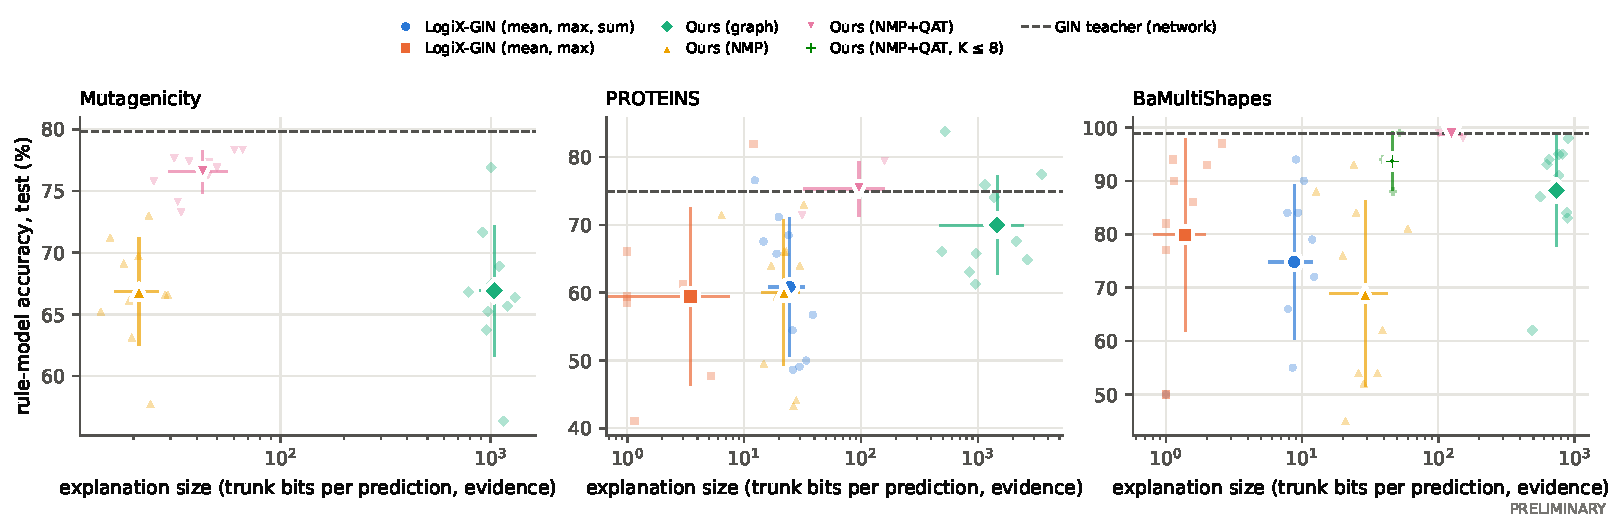
\includegraphics[width=\textwidth]{figures/fig_pareto.pdf}%
  }{\fbox{\parbox[c][4cm]{0.95\textwidth}{\centering\todo{fig\_pareto.pdf: rule-model accuracy vs explanation size}}}}
  \caption{Accuracy of the rule model against the size of its explanations (trunk bits
    per prediction, log scale), test split, one small dot per fold and the mean $\pm$ std
    per model. Dashed line: \teacher{}. Up and to the left is better.}
  \label{fig:pareto}
\end{figure*}


% =====================================================================================
% table_sanity.tex: model-randomisation sanity check of the explanations (Q2; Adebayo et
%   al., "Sanity checks for saliency maps", NeurIPS 2018).
%
% Question: do the explanations, and above all their ground-truth precision, depend on
%   what the model learned? A GT precision that a model with scrambled weights also
%   reaches measures the dataset (how many nodes lie near an NO2 group), not the model.
% Protocol (utils/sanity.py, sanity_randomisation.py, feat/paper-figures 82edfda):
%   independent randomisation, one stage at a time with every other stage trained: head,
%   prototypes, conv layer 2, 1, 0. Randomise = permute the entries of every trained
%   parameter tensor of the stage (same values, scale and sparsity; learned assignment
%   destroyed). 3 draws per stage and fold, test split, evidence explanations.
%   Not the cascade (cumulative) order: a permuted head alone already predicts one class
%   on every graph (NMP and QAT NMP Mutagenicity), so the lower stages say nothing more.
%   Not re-initialisation: Phi initialises to w=1, b=0, i.e. every literal constant true,
%   so a re-initialised head cites nothing (an artefact of the init).
%   Columns: rule-model accuracy; Agree.: same predicted class as the trained model;
%   Jacc.: Jaccard of the cited node sets, over graphs where both cite a node; GT prec.
%   of the randomised model (chance in brackets).
%   Command: python sanity_randomisation.py --run_path results_final/<exp>/<ds>/<model>/fold*
%   (CPU, ~5 s per fold and draw; 10 folds x 3 draws x 2 models ~ 10 min).
%
% Smoke run (fold 3, 3 draws, 2026-10-21; preliminary pre-head-fix runs):
%   NMP Mutagenicity (sum_ablation_ctrl), trained: rule acc 63.1, GT prec. 78 (chance 24)
%     randomised    rule acc   agree   Jacc.   GT prec.
%     head            47.3     0.39    0.54     20
%     prototypes      55.3     0.36    0.19     37
%     conv2           45.7     0.65    0.15     13 (n=3)
%     conv1           55.4     0.36    0.19     22
%     conv0           57.1     0.43    0.16     22
%   -> passes: explanations change with every stage, GT precision falls to chance.
%   QAT NMP Mutagenicity (qat_nmp) fold 3: inconclusive, the trained model's evidence
%     cites a node in only 10% of test graphs (19 GT-scored), the randomised ones in ~0%.
%
% What it shows: that the explanations and their GT precision come from the learned
%   weights of every stage, not from the data alone.
% What it does not show: that the explanations are correct or useful (a pass is
%   necessary, not sufficient); the data-randomisation test (retrain on permuted labels,
%   GPU) is not run.
%
% STATUS: code ready, smoke run only. \tbd.
% TODO:
%   [ ] run on the final E1 folds of every node-prototype and classic model with a GT
%       region (Mutagenicity, BA2Motifs, BAMultiShapes); fill from sanity_*.json.
%   [ ] decide: data-randomisation test (permuted labels, one retraining per fold).
% =====================================================================================
\begin{table}[t]
  \centering
  \caption{Model-randomisation sanity check on Mutagenicity (test, mean over folds and 3
    draws). One stage at a time has its trained parameters permuted. Agree.: same class as
    the trained model. Jacc.: overlap of the cited nodes with the trained model's. GT
    prec.: cited nodes in the ground truth (\%, chance in brackets).}
  \label{tab:sanity}
  \small
  \begin{tabular}{llcccc}
    \toprule
    Model & Randomised & Rule acc.\ (\%) & Agree.\ (\%) & Jacc. & GT prec.\ (\%) \\
    \midrule
    \multirow{6}{*}{\oursnmp{}}
      & none (trained) & \tbd & 100 & 1 & \tbd \\
      & head           & \tbd & \tbd & \tbd & \tbd \\
      & prototypes     & \tbd & \tbd & \tbd & \tbd \\
      & conv layer 2   & \tbd & \tbd & \tbd & \tbd \\
      & conv layer 1   & \tbd & \tbd & \tbd & \tbd \\
      & conv layer 0   & \tbd & \tbd & \tbd & \tbd \\
    \midrule
    \multirow{6}{*}{\oursqat{}}
      & none (trained) & \tbd & 100 & 1 & \tbd \\
      & head           & \tbd & \tbd & \tbd & \tbd \\
      & prototypes     & \tbd & \tbd & \tbd & \tbd \\
      & conv layer 2   & \tbd & \tbd & \tbd & \tbd \\
      & conv layer 1   & \tbd & \tbd & \tbd & \tbd \\
      & conv layer 0   & \tbd & \tbd & \tbd & \tbd \\
    \bottomrule
  \end{tabular}
\end{table}


\todo{results paragraph: fidelity of the rule model; QAT closes the gap to 100\%; size of
explanations vs classic \logix{}; ground-truth precision vs chance and vs competitors; randomisation check
(\cref{tab:sanity}).}

% -------------------------------------------------------------------------------------
\subsection{Ablations (Q3)}
\label{sec:exp:ablation}

\paragraph{Components of the node prototypes.}
% =====================================================================================
% table_nmp_components.tex: what each component of the node prototypes brings (Q3;
%   Notion E5, P0).
%
% Question: NMP = node-level binary prototypes + care mask + push onto real nodes
%   (+ optional vocab_reg). Which component gives the accuracy, which gives the short /
%   correct explanations?
% Protocol (to write): ONE tuned NMP set per dataset (the E1 best set), then switch the
%   components off one at a time, 10 folds each, same teachers and folds. Rows add the
%   components cumulatively:
%     node prototypes, dense  train_proto.py --proto_level node, --push_every 0, no mask
%     + push                  --push_every <best>
%     + care mask             --proto_mask (mask_reg, mask_anneal_frac 0.8)  [= NMP]
%     + vocab_reg             --vocab_reg 0.1  (only if not already in the best set)
%     + QAT                   qat_proto.py   [= NMP+QAT]
%   plus the head-saturation fix on / off (--head_init center --logit_loss) as one row or
%   an appendix line, since it changed MUTAG NMP from collapsed to working.
% Metrics: test balanced acc., rule-model acc., fidelity, explanation bits, GT precision.
% What it should show: push makes prototypes real nodes (readable cards); the mask makes
%   explanations short (bits); QAT makes them faithful.
% What it will not show: interactions beyond the cumulative order (no full factorial).
%
% STATUS: NOT RUN. Code needed: an experiment YAML (e.g.
%   configs/experiments/nmp_components.yaml) with params_from: <every variant>:
%   node_mask_push, and the variants as model entries in configs/models.yaml (fixed
%   args only). Compute: 10 folds × 5 variants × 3 datasets = 150 runs (estimate
%   before launching).
% Datasets: MUTAG, PROTEINS, Mutagenicity (Notion E5); BAMultiShapes for GT precision.
% TODO:
%   [ ] model entries + YAML, smoke test (1 fold, few epochs), then estimate, then run.
% =====================================================================================
\begin{table}[t]
  \centering
  \caption{Components of the node prototypes, added one at a time with the tuned \nmp{}
    set (test, 10 folds, \%). Bits: explanation size. GT prec.: on Mutagenicity.}
  \label{tab:nmp_components}
  \small
  \setlength{\tabcolsep}{3pt}
  \begin{tabular}{lcccccc}
    \toprule
    & \multicolumn{2}{c}{MUTAG} & \multicolumn{2}{c}{PROTEINS} & \multicolumn{2}{c}{Mutagenicity} \\
    \cmidrule(lr){2-3}\cmidrule(lr){4-5}\cmidrule(lr){6-7}
    Variant & Rule acc. & Bits & Rule acc. & Bits & Rule acc. & GT prec. \\
    \midrule
    node prototypes (dense)  & \tbd & \tbd & \tbd & \tbd & \tbd & \tbd \\
    + push                   & \tbd & \tbd & \tbd & \tbd & \tbd & \tbd \\
    + care mask (= \oursnmp{})   & \tbd & \tbd & \tbd & \tbd & \tbd & \tbd \\
    + vocabulary penalty     & \tbd & \tbd & \tbd & \tbd & \tbd & \tbd \\
    + QAT (= \oursqat{})     & \tbd & \tbd & \tbd & \tbd & \tbd & \tbd \\
    \midrule
    \nmp{} without head fix  & \tbd & \tbd & \tbd & \tbd & \tbd & \tbd \\
    \bottomrule
  \end{tabular}
\end{table}

\todo{paragraph}

\paragraph{Binarisation: from a soft network to its rules.}
% =====================================================================================
% table_binarisation.tex: closing the gap between the soft network and its rules (Q3;
%   Notion E6 fidelity hardening + the QAT study, docs/QAT.md).
%
% Question: the network computes with soft truth values; a reader gets the rules
%   (every bit binarised at 0.5). Fidelity of a trained NMP student is ~74-80%. Which
%   fine-tune makes the network equal to its rules at the smallest accuracy cost?
% Arms (all start from the same trained NMP student):
%   none            the trained student, read as rules
%   sharpen (train) train_proto.py --harden_to 30: sigmoids sharpened during training
%   sharpen FT      harden_proto.py: gradual sharpening fine-tune, beta 1 -> 20, 300 or
%                   1000 epochs
%   hard FT         every bit binarised at once, straight-through, then fine-tuned
%   QAT             qat_proto.py: Quant-Noise, binarised share ramps 0 -> 1 over 2/3 of
%                   the epochs, STE on binarised bits, keeps the epoch with the best
%                   validation rule-model accuracy; "tuned" = student and QAT tuned jointly
%                   by Optuna on the rule-model val balanced accuracy (node_mask_push_qat)
% Metrics: test; network accuracy, fidelity, rule-model accuracy (%), explanation bits.
%
% Sources:
%   rows "seeds 0-2": Mutagenicity NMP, results_proto/Mutagenicity/node-facbe6d14f72,
%     RANDOM split (not the k-fold), seeds 0-2, 2026-10-12/13 (docs/QAT.md table; memory
%     paper-todo). Preliminary protocol: the final table must use the k-fold folds.
%   rows "10 folds": results_final/sum_ablation_ctrl/Mutagenicity/node_mask_push (none)
%     and results_final/qat_nmp/Mutagenicity/node_mask_push_qat (QAT tuned).
% What it shows: sharpening and hard fine-tunes reach fidelity ~0.9-1 but lose 5-11 points
%   of network accuracy and do not improve the rules; progressive QAT gives the best rule
%   model (+10 points over the rules of the untouched student on 10 folds, 10/10 folds) at
%   fidelity 1; the price is 4 points of network accuracy and 2x longer explanations (evidence bits
%   43 vs 21; plain counts 61 vs 24).
% What it does not show: whether the rule-model gain holds on the other datasets (PROTEINS
%   folds 0-2: rules 75.3 vs 67.9; BAMultiShapes: see table_num_prototypes.tex). Bits are
%   evidence bits (table_interp.tex): QAT makes 92% of the head literals constant, and with
%   them left out its explanations still cite a node in only 35% of the Mutagenicity GT
%   predictions (NMP 82%).
%
% STATUS: \prelim. Mixed protocols (random-split seeds vs k-fold folds).
% TODO:
%   [ ] rerun every arm on the 10 k-fold folds of the FINAL E1 NMP students (post-hoc
%       fine-tunes from the final checkpoints, no retraining): harden_proto.py (1000 ep),
%       hard FT, qat_proto.py with a fixed set, + the jointly tuned QAT of E1.
%   [ ] at least Mutagenicity + PROTEINS + BAMultiShapes; same columns + GT precision.
%   [ ] fig_binarisation.tex plots the same runs (val curves).
% =====================================================================================
\begin{table}[t]
  \centering
  \caption{Binarisation of a trained \nmp{} student on Mutagenicity (test, \%): network
    accuracy, fidelity of its rules, accuracy of the rule model, explanation size.
    \prelim{Grey}: preliminary runs (rows ``seeds 0--2'' on a random split).}
  \label{tab:binarisation}
  \small
  \setlength{\tabcolsep}{3.5pt}
  \begin{tabular}{llcccc}
    \toprule
    Runs & Fine-tune & Network acc. & Fid. & Rule acc. & Bits \\
    \midrule
    \multirow{6}{*}{seeds 0--2}
      & none                          & \prelim{81.2} & \prelim{80} & \prelim{72.7} & \tbd \\
      & sharpen during training ($\beta$ 30) & \prelim{76.9} & \prelim{88} & \prelim{71.6} & \tbd \\
      & sharpen FT, 300 ep            & \prelim{70.1} & \prelim{88} & \prelim{67.2} & \tbd \\
      & sharpen FT, 1000 ep           & \prelim{76.3} & \prelim{90} & \prelim{74.1} & \tbd \\
      & hard FT (all bits at once)    & \prelim{69.7} & \prelim{100} & \prelim{69.7} & \tbd \\
      & QAT, 300 ep                   & \prelim{74.2} & \prelim{100} & \prelim{\ms{74.2}{5.7}} & \tbd \\
    \midrule
    \multirow{5}{*}{10 folds}
      & none                          & \prelim{\ms{80.4}{2.1}} & \prelim{\ms{73.6}{5.9}} & \prelim{\ms{66.8}{4.3}} & \prelim{\ms{21}{5}} \\
      & sharpen FT, 1000 ep           & \tbd & \tbd & \tbd & \tbd \\
      & hard FT                       & \tbd & \tbd & \tbd & \tbd \\
      & QAT, fixed set                & \tbd & \tbd & \tbd & \tbd \\
      & QAT, tuned with the student   & \prelim{\ms{76.6}{1.7}} & \prelim{\ms{100}{0}} & \prelim{\ms{76.6}{1.7}} & \prelim{\ms{43}{13}} \\
    \bottomrule
  \end{tabular}
\end{table}

% =====================================================================================
% fig_binarisation.tex: how the binarisation methods move a student from soft network
%   to rule model (Q3; companion of table_binarisation.tex).
%
% What the experiment tests: starting from the same trained NMP student, each fine-tune
%   (sharpening schedule, hard fine-tune, progressive QAT) is meant to make the network
%   compute its rules. We track, over the fine-tuning epochs, the validation accuracy of
%   the soft network and of the rule model (every bit binarised).
% Plot: left, validation accuracy vs epoch, one colour per method, solid = rule model,
%   dashed = soft network (they meet when fidelity reaches 1); QAT also shows its
%   binarised share (rate) on a secondary axis. Right, final test point per method in the
%   plane (network accuracy, rule-model accuracy), diagonal = fidelity 1, mean ± std over
%   folds.
% What it shows: sharpening kills the gradient (a TELL unit passes it only for |z| <
%   0.034 at beta 30) so accuracy drops before fidelity rises; binarising all bits at
%   once loses ~11 points in one step; QAT's progressive random share keeps the soft
%   gradients of the other bits and lands on the diagonal with the best rule model.
% What it does not show: why the QAT rule model plateaus (~77% on Mutagenicity; the
%   binary prototype head is the suspected ceiling, docs/QAT.md); other datasets unless
%   added as panels.
% Data: qat.json (per-epoch history: qat/val_acc_soft, qat/val_acc_rules, qat/rate) and
%   MLflow qat/<dataset>; harden_proto.py histories (MLflow finetune/harden). Must come
%   from the k-fold reruns listed in table_binarisation.tex, not from the random-split
%   seeds.
% GENERATED BY: python plot_paper.py binarisation   (sources: configs/paper_figures.yaml, code:
%   utils/paper_figures.py, branch feat/paper-figures). "preliminary: true" in the config
%   stamps PRELIMINARY on the figure; set it to false only when every source is final.
% STATUS: PRELIMINARY version drawn 2026-10-21: only the QAT arm (qat_nmp, 10 folds) and the untouched NMP; the sharpening / hard fine-tune arms appear once their k-fold runs exist (harden.json is read automatically).
% TODO:
%   [ ] reruns, then the plotting script -> paper/figures/fig_binarisation.pdf.
% =====================================================================================
\begin{figure}[t]
  \centering
  \IfFileExists{figures/fig_binarisation.pdf}{%
    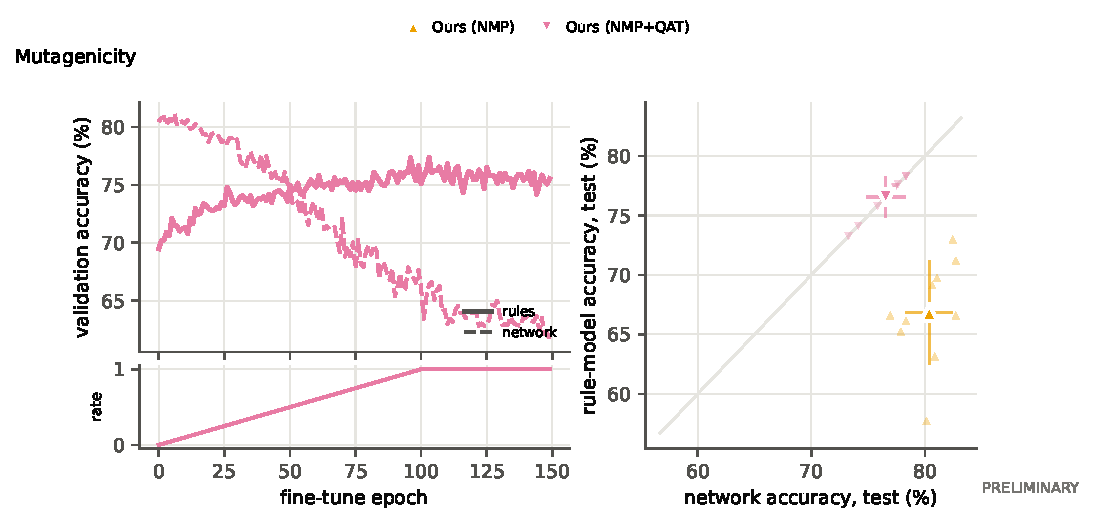
\includegraphics[width=\linewidth]{figures/fig_binarisation.pdf}%
  }{\fbox{\parbox[c][4cm]{0.95\linewidth}{\centering\todo{fig\_binarisation.pdf: soft vs rule accuracy per fine-tune}}}}
  \caption{Binarisation fine-tunes of an \nmp{} student on Mutagenicity. Left: validation
    accuracy of the soft network (dashed) and of its rules (solid) during the
    fine-tune. Right: final test accuracies; on the diagonal the network computes exactly
    its rules.}
  \label{fig:binarisation}
\end{figure}

\todo{paragraph}

\paragraph{Number of prototypes.}
% =====================================================================================
% table_num_prototypes.tex: how many prototypes does the QAT NMP student need? (Q3)
%
% Question: with 32-64 prototypes most of them end up with no cared bit (constant
%   similarity 1; Mutagenicity qat_nmp fold 1: 25/32 prototypes, all head weights 0),
%   and explanations cite many prototypes. Does a small K keep the accuracy and shorten
%   the explanations?
% Protocol: node_mask_push_qat with num_prototypes restricted (search space nmp_qat_p8 =
%   {4, 8}, nmp_qat_p16 = {8, 16}; nmp_qat = {16, 32, 64}), 15 Optuna trials on fold 0
%   (25 for qat_nmp), then folds 0-2. The K column is the value the search picked.
%   Test, mean ± std over folds 0-2.
% Sources (results_final/<exp>/<dataset>/node_mask_push_qat*/fold{0,1,2}):
%   BAMultiShapes K=8: qat_nmp_p8_3fold;  K=64: qat_nmp_3fold.
%   Mutagenicity  K=32: qat_nmp folds 0-2;  K in {8,16}: qat_nmp_p16_3fold (RUNNING since
%     2026-10-21 10:25, expected done ~18:00).
%   PROTEINS K=32: qat_nmp_3fold.
% What it shows (BAMultiShapes, evidence sizes): K=8 cuts explanations ~3x (bits 46 vs
%   125, 4 vs 26 prototypes cited) and raises GT precision (99 vs 87) for -5 points of
%   accuracy. (Plain counts, constant literals included: 71 vs 339 bits, 88 vs 78 GT.)
% What it does not show: 3 folds only (std is large: K=8 folds are 99/88/94); the search
%   ran on fold 0 only; K and the other hyper-parameters change together (each K row is
%   its own study), so this is "best model with at most K", not a pure K effect.
%
% STATUS: partially filled, \prelim (3 folds).
% TODO:
%   [ ] Mutagenicity K in {8,16} when qat_nmp_p16_3fold finishes.
%   [ ] decide the paper's K policy (fixed small K, or K in the search) and, if kept,
%       run 10 folds for the chosen rows; else move to the appendix.
%   [x] evidence-only explanation size (interp rerun 2026-10-21, *_evidence columns,
%       folds 0-2 of each source). Mutagenicity K=32 GT prec.: only 5 of 295 scored
%       predictions keep a node in their evidence (folds 0, 1: none), one fold -> 2%.
% =====================================================================================
\begin{table}[t]
  \centering
  \caption{\nmpqat{} with a bounded number of prototypes $K$ (test, folds 0--2, mean
    $\pm$ std). Bal.\ acc.\ of the network (= rule model). Lit./Bits: explanation size.
    Protos: prototypes cited. GT prec.: cited nodes in the ground truth (\%). Sizes count input-dependent literals only. $^\ast$: 5 of 295 scored predictions cite a node (one fold).
    \prelim{Grey}: preliminary runs.}
  \label{tab:num_prototypes}
  \small
  \setlength{\tabcolsep}{3.5pt}
  \begin{tabular}{lccccccc}
    \toprule
    Dataset & $K$ space & $K$ & Bal.\ acc. & Lit. & Bits & Protos & GT prec. \\
    \midrule
    \multirow{2}{*}{BAMultiShapes}
      & \{4, 8\}       & 8  & \prelim{\ms{93.7}{5.5}} & \prelim{\ms{3.1}{1.3}}  & \prelim{\ms{46}{7}}   & \prelim{\ms{4.0}{1.0}}  & \prelim{\ms{99}{1}} \\
      & \{16, 32, 64\} & 64 & \prelim{\ms{98.7}{0.6}} & \prelim{\ms{11.0}{0.5}} & \prelim{\ms{125}{26}} & \prelim{\ms{26.0}{3.0}} & \prelim{\ms{87}{17}} \\
    \midrule
    \multirow{2}{*}{Mutagenicity}
      & \{8, 16\}      & \tbd & \tbd & \tbd & \tbd & \tbd & \tbd \\
      & \{16, 32, 64\} & 32 & \prelim{\ms{76.0}{2.7}} & \prelim{\ms{2.6}{0.6}} & \prelim{\ms{42}{16}} & \prelim{\ms{7.0}{2.0}} & \prelim{2}$^\ast$ \\
    \midrule
    \multirow{2}{*}{PROTEINS}
      & \{8, 16\}      & \tbd & \tbd & \tbd & \tbd & \tbd & \na \\
      & \{16, 32, 64\} & 32 & \prelim{\ms{72.7}{4.9}} & \prelim{\ms{4.4}{3.4}} & \prelim{\ms{96}{64}} & \prelim{\ms{10.7}{6.7}} & \na \\
    \bottomrule
  \end{tabular}
\end{table}

\todo{paragraph}

\paragraph{Sum pooling.}
% =====================================================================================
% table_sum_ablation.tex: does a sum readout help the prototype students? (Q3; Notion E2)
%
% Question: classic LogiX-GIN reads mean | max | sum pooled units. Sum-pooled values are
%   unbounded counts (no 1 - s negation; at graph level they are thresholded by phi_sum
%   before the prototypes). Does adding sum change accuracy or the explanations?
% Protocol (controlled, configs/experiments/sum_ablation_ctrl.yaml): each *_sum model is
%   trained with the best set of its no-sum twin (params_from), so a pair differs ONLY by
%   --pool_ops; same teachers and folds. Paired over the 10 folds: mean difference
%   (with sum - without), folds where sum is better, two-sided Wilcoxon signed-rank p.
%   PROTEINS / BAMultiShapes: Optuna set of the no-sum model (sum_ablation study, fold 0);
%   Mutagenicity: hand-tuned set (best_sets), no study.
% Source: results_final/sum_ablation_ctrl/<dataset>/<model>/fold<k>/{final,interp}.json;
%   computed 2026-10-21 by a scratchpad script (paired Wilcoxon, scipy). The no-sum folds
%   of PROTEINS / BAMultiShapes are the sum_ablation runs (symlinks).
% What it shows: at equal hyper-parameters sum does not change accuracy (|Δ| ≤ 1.4
%   points), the drop seen in sum_ablation came from the different Optuna sets. Sum
%   always makes explanations longer (bits). It lowers graph-level fidelity on PROTEINS
%   (-23 points, 0/10 folds better) but not on Mutagenicity; NMP is neutral.
% What it does not show: why graph-level fidelity drops on PROTEINS (the phi_sum
%   thresholds of counts are the lead; trunk and head fidelity are unchanged); whether
%   sum would help with a set tuned for it; MUTAG (left out, unstable).
%
% STATUS: filled (2026-10-21) but trained BEFORE the head-saturation fix (2026-10-19).
%   Both arms of each pair lack it, so the comparison is internally fair; mark \prelim
%   until decided whether to rerun.
% TODO:
%   [ ] decide: keep as is (fair pairs) or rerun with the fixed models (≈80 runs,
%       ≤1.0 kgCO2e last time).
%   [ ] add the diagnosis row if found (phi_sum thresholds at graph level).
%   [ ] maybe move to the appendix: the paper's models all drop sum.
% =====================================================================================
\begin{table}[t]
  \centering
  \caption{Effect of adding a sum readout at equal hyper-parameters (with sum $-$
    without, test, paired over 10 folds; in brackets: folds where sum is better, Wilcoxon
    $p$). Accuracy is balanced accuracy; Fid.\ and Rule acc.\ are in points; Bits is the
    explanation size.}
  \label{tab:sum_ablation}
  \small
  \setlength{\tabcolsep}{3pt}
  \begin{tabular}{llcccc}
    \toprule
    Dataset & Model & $\Delta$ Bal.\ acc. & $\Delta$ Fid. & $\Delta$ Rule acc. & $\Delta$ Bits \\
    \midrule
    \multirow{2}{*}{PROTEINS}
      & graph & \prelim{$-1.4$ (3, .38)} & \prelim{$\mathbf{-23.0}$ (0, .002)} & \prelim{$\mathbf{-11.6}$ (1, .004)} & \prelim{$+463$ (7, .06)} \\
      & \nmp{} & \prelim{$-0.2$ (5, .85)} & \prelim{$+8.4$ (7, .19)} & \prelim{$+4.1$ (7, .27)} & \prelim{$\mathbf{+30}$ (10, .002)} \\
    \midrule
    \multirow{2}{*}{BAMultiShapes}
      & graph & \prelim{$+0.4$ (5, .34)} & \prelim{$-10.0$ (2, .16)} & \prelim{$-9.8$ (2, .10)} & \prelim{$\mathbf{+684}$ (10, .002)} \\
      & \nmp{} & \prelim{$+0.7$ (4, .34)} & \prelim{$+3.6$ (6, .70)} & \prelim{$+3.7$ (6, .63)} & \prelim{$\mathbf{+42}$ (9, .006)} \\
    \midrule
    \multirow{2}{*}{Mutagenicity}
      & graph & \prelim{$\mathbf{-1.2}$ (1, .004)} & \prelim{$-0.8$ (3, .28)} & \prelim{$-0.2$ (4, .83)} & \prelim{$\mathbf{+502}$ (9, .004)} \\
      & \nmp{} & \prelim{$+1.0$ (8, .13)} & \prelim{$-1.7$ (3, .50)} & \prelim{$+0.3$ (6, .90)} & \prelim{$+4$ (7, .13)} \\
    \bottomrule
  \end{tabular}
\end{table}

\todo{paragraph}

\paragraph{Readable trunk: layer-wise sparsification.}
% =====================================================================================
% table_hoyer.tex: can the trunk be made readable? Layer-wise Hoyer sparsification
%   (Q3; Notion E7).
%
% Question: only conv layer 0 decodes to short rules (~3 literals); a unit of layers 1-2
%   has ~1e10 minimal covers (DNF terms) and needs 10-14 literals. Does the layer-wise
%   Hoyer fine-tune of LogiX-GIN (sparsify_proto.py: head, then convs last to first, each
%   step accepted only if validation accuracy holds), ported to prototype students, make
%   the trunk readable without losing accuracy or fidelity?
% Protocol: sparsify_proto.py with low learning rates for L0/L1 (--conv_lr 5e-4 5e-4
%   5e-3, lw_max_epochs 1000) on the final NMP folds; dense = the same checkpoint.
% Metrics (test): network acc., fidelity, rule acc., explanation bits; per conv layer:
%   median nonzero weights per unit (nz), dead units (no nonzero weight), median number of
%   minimal covers of a unit (min_covers.count_min_covers) and median shortest rule length
%   (greedy minimum-cardinality bound, exact).
% Sources: Mutagenicity = results_final/sum_ablation_ctrl/Mutagenicity/node_mask_push
%   (hand-tuned set), PROTEINS = results_final/sum_ablation/PROTEINS/node_mask_push
%   (Optuna set); queue 2026-10-15/16, logs/hoyer_lowlr_kfold/; numbers from the
%   scratchpad comparison script of session 72b5e02d (hoyer_kfold_compare.json), memory
%   paper-todo 2026-10-16. Rerun with a committed script before the final version.
% What it shows: accuracy unchanged, fidelity -3.6 points (2/10 folds better, p 0.09);
%   L1 goes from ~5e10 covers per unit to ~6, but much of the "sparsity" is dead units
%   (L1 28%, L2 72%); explanation size barely moves (24 -> 22 bits). PROTEINS: nothing
%   moves. So Hoyer makes the trunk readable, not the explanations shorter.
% What it does not show: whether a reader can use the L1/L2 rules; QAT students (not run).
%
% STATUS: \prelim (pre head-fix students, scratchpad script); PROTEINS layer columns partial.
% TODO:
%   [ ] post-hoc stage in the experiment YAML (sparsify + rule counts), on the final E1
%       NMP and NMP+QAT folds; guard unpack_rules with the min-cover bound first (63 GB
%       blow-up on Mutagenicity fold 5).
%   [ ] decide main text vs appendix (negative-ish result).
%   [ ] RULE COUNTS ARE UPPER BOUNDS (audit 2026-10-22, issue 7). covers/unit
%       (min_covers.count_min_covers, rule_eval.rule_stats) counts the minimal covers of the
%       threshold over free literals, but a literal and its negation read the same
%       neighbourhood count and periodic literals are bands, so some covers can never be
%       satisfied. Planned fix: one forward pass on the TRAINING set, record which literals
%       are ever true (and which pairs co-occur), drop the literals never activated before
%       counting, and report only the rules that can fire on data. (The authors' notebook
%       already drops literals true on every graph and filters by min_support on the
%       activations: nbs/LayerWiseRules.ipynb cells 9, 34.)
% =====================================================================================
\begin{table}[t]
  \centering
  \caption{Layer-wise Hoyer sparsification of the \nmp{} trunk (test, 10 folds, medians
    over units). nz: nonzero weights per unit (L0/L1/L2). Covers: minimal covers (DNF terms) of
    an L1 unit. Dead: L1/L2 units with no nonzero weight.
    \prelim{Grey}: preliminary runs.}
  \label{tab:hoyer}
  \small
  \setlength{\tabcolsep}{3pt}
  \begin{tabular}{llcccccc}
    \toprule
    Dataset & Trunk & Acc. & Fid. & Bits & nz L0/L1/L2 & Covers L1 & Dead L1/L2 \\
    \midrule
    \multirow{2}{*}{Mutagenicity}
      & dense & \prelim{80.4} & \prelim{73.6} & \prelim{24} & \prelim{15/48/45} & \prelim{$5{\times}10^{10}$} & \prelim{--} \\
      & Hoyer & \prelim{81.1} & \prelim{70.0} & \prelim{22} & \prelim{10/20/4}  & \prelim{6}  & \prelim{28\%/72\%} \\
    \midrule
    \multirow{2}{*}{PROTEINS}
      & dense & \prelim{74.2} & \prelim{65.2} & \tbd & \tbd/\tbd/\prelim{45} & \tbd & \tbd \\
      & Hoyer & \prelim{73.4} & \prelim{66.7} & \tbd & \tbd/\tbd/\prelim{32} & \tbd & \tbd \\
    \bottomrule
  \end{tabular}
\end{table}

% =====================================================================================
% fig_rule_complexity.tex: how complex is each trunk unit as a rule, per layer (Q3;
%   companion of table_hoyer.tex; the depth limit of CLAUDE.md "rule-extraction limits").
%
% What the experiment tests: each conv unit is a threshold over binary literals; its
%   exact DNF is the set of its minimal covers. We measure, per unit, (a) the length of
%   its shortest rule (greedy minimum-cardinality bound, exact) and (b) the number of
%   its minimal covers (min_covers.count_min_covers; never enumerate a unit with ~1e10
%   covers), for the dense trunk and after layer-wise Hoyer, per layer L0 / L1 / L2.
% Plot: two panels. Left: shortest rule length per unit (box or violin per layer, dense
%   vs Hoyer side by side). Right: number of minimal covers per unit (log scale, same
%   layout). Dead units (no nonzero weight) shown as a separate count above each Hoyer box.
% What it shows: only L0 decodes to short rules (~3 literals); L1/L2 units need ~10-14
%   literals and have ~1e10 covers (weight diffusion, not a search limit); Hoyer brings L1
%   down to a few covers, partly by killing units.
% What it does not show: the explanation size of a prediction (that is set by the head
%   and the prototypes' cared bits, table_interp.tex); semantic quality of the rules.
% Data: final NMP (and NMP+QAT) checkpoints of E1, dense and after sparsify_proto.py;
%   min_covers.py on every unit.
% GENERATED BY: python plot_paper.py rule_complexity   (sources: configs/paper_figures.yaml, code:
%   utils/paper_figures.py, branch feat/paper-figures). "preliminary: true" in the config
%   stamps PRELIMINARY on the figure; set it to false only when every source is final.
% STATUS: PRELIMINARY version drawn 2026-10-21 (sum_ablation_ctrl NMP, 10 folds, dense vs low-lr layer-wise Hoyer). Final after E1 + the Hoyer post-hoc stage.
% TODO:
%   [ ] committed script computing per-unit bound + cover count (cheap, exact; guard
%       against enumeration) -> json per fold -> paper/figures/fig_rule_complexity.pdf.
%   [ ] appendix if table_hoyer goes to the appendix.
% =====================================================================================
\begin{figure}[t]
  \centering
  \IfFileExists{figures/fig_rule_complexity.pdf}{%
    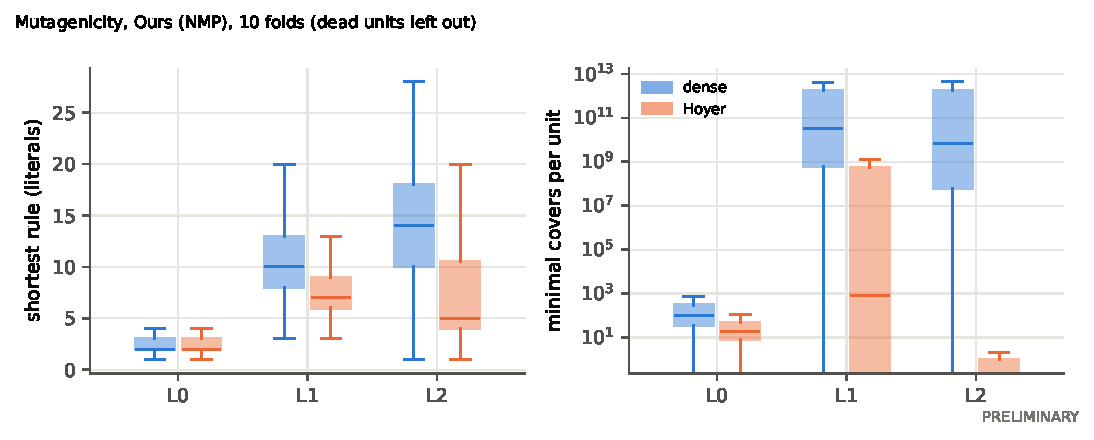
\includegraphics[width=\linewidth]{figures/fig_rule_complexity.pdf}%
  }{\fbox{\parbox[c][4cm]{0.95\linewidth}{\centering\todo{fig\_rule\_complexity.pdf: rule length and covers per layer}}}}
  \caption{Complexity of the trunk units as rules, per conv layer, for the dense trunk and
    after layer-wise Hoyer sparsification (Mutagenicity, \nmp{}, all folds). Left: length of
    the shortest rule. Right: number of minimal covers (DNF terms), log scale.}
  \label{fig:rule_complexity}
\end{figure}

\todo{paragraph; or move to the appendix if the trunk result stays negative}

% -------------------------------------------------------------------------------------
\subsection{Qualitative results (Q4)}
\label{sec:exp:qualitative}

% =====================================================================================
% fig_agreement.tex: do the prototypes separate the classes? (Q4; Notion E8)
%
% What the experiment tests: for each prototype, the distribution of its agreement
%   (Hamming similarity on cared bits; for node prototypes, of the best-matching node of
%   each graph) over the training graphs, one histogram per class. A prototype is useful
%   if its agreement separates the classes; separation = |2 AUC - 1| of the agreement as
%   a class score.
% Plot: one row per dataset (Mutagenicity, BAMultiShapes), the prototypes cited by the
%   head (with at least one cared bit), sorted by separation; per prototype a small step
%   histogram per class, separation and cared bits in the title. (Head thresholds as
%   vertical lines: not drawn yet.)
% What it shows: which prototypes carry the decision and how cleanly; that prototypes
%   with no cared bit are constant (agreement 1 for every graph) and are hidden.
% What it does not show: what the prototype means (fig_prototypes.tex); whether the head
%   uses it alone or in combination (fig_explanation.tex); stability across folds.
% Data: agreement.{png,json,npz} written by every train_proto.py run (utils/agreement.py)
%   and by the explorer (explorer/, same computation); one chosen fold per dataset of the
%   final NMP+QAT run (say which fold, and pick it by a stated rule, e.g. median test
%   accuracy, not the best-looking one).
% GENERATED BY: python plot_paper.py agreement   (sources: configs/paper_figures.yaml, code:
%   utils/paper_figures.py, branch feat/paper-figures). "preliminary: true" in the config
%   stamps PRELIMINARY on the figure; set it to false only when every source is final.
% STATUS: PRELIMINARY version drawn 2026-10-21 (qat_nmp fold 7 on Mutagenicity, qat_nmp_3fold on BAMultiShapes, representative folds). Final after E1.
% TODO:
%   [ ] choose fold rule; plotting script -> paper/figures/fig_agreement.pdf.
%   [ ] mean-pooled agreement variant for NMP (BAMultiShapes max-agreement plot was
%       uninformative, todo P1).
% =====================================================================================
\begin{figure*}[t]
  \centering
  \IfFileExists{figures/fig_agreement_Mutagenicity.pdf}{%
    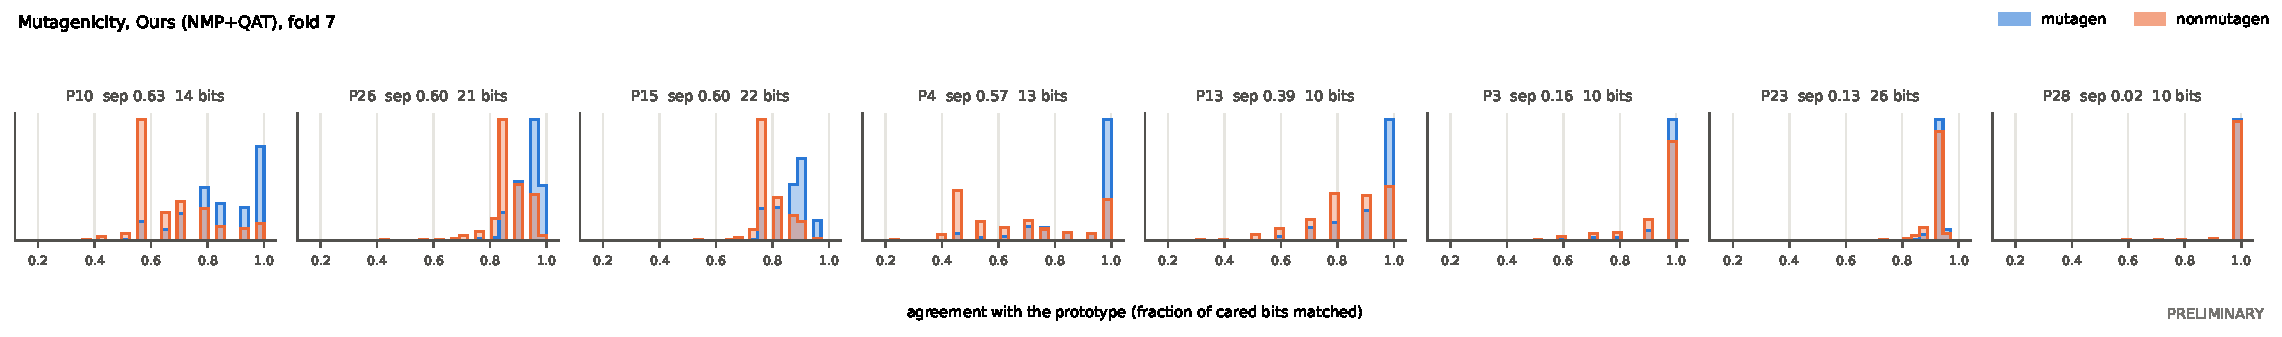
\includegraphics[width=\textwidth]{figures/fig_agreement_Mutagenicity.pdf}%
  }{\fbox{\parbox[c][3cm]{0.95\textwidth}{\centering\todo{fig\_agreement\_Mutagenicity.pdf}}}}\\[4pt]
  \IfFileExists{figures/fig_agreement_BaMultiShapes.pdf}{%
    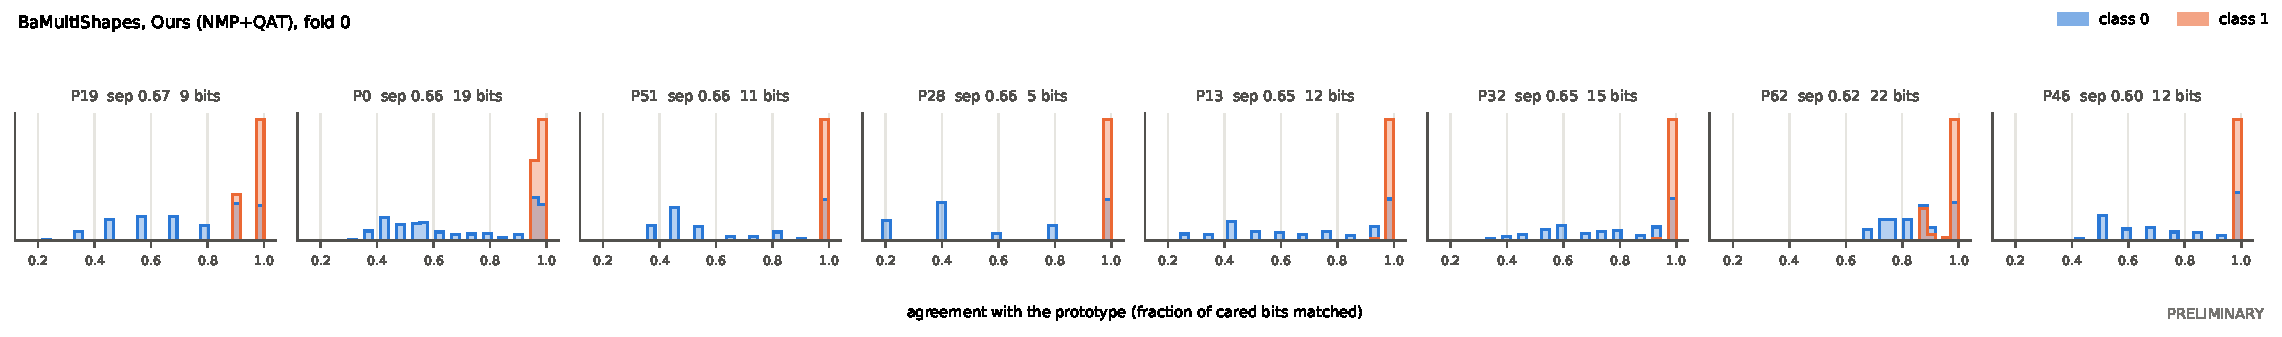
\includegraphics[width=\textwidth]{figures/fig_agreement_BaMultiShapes.pdf}%
  }{\fbox{\parbox[c][3cm]{0.95\textwidth}{\centering\todo{fig\_agreement\_BaMultiShapes.pdf}}}}\\[4pt]
  \caption{Agreement of the training graphs with each prototype cited by the explanations
    (best matching node, share of the cared bits that match), one histogram per class,
    prototypes by decreasing class separation $|2\,\mathrm{AUC}-1|$ (title, with the number
    of cared bits). Representative fold (median test balanced accuracy).}
  \label{fig:agreement}
\end{figure*}

% =====================================================================================
% fig_prototypes.tex: what the prototypes are (Q4; Notion E11 qualitative figures).
%
% What the experiment tests: after push, each node prototype is a real training node; its
%   cared bits are trunk units, each decodable (at least for L0) into a rule over the
%   node's neighbourhood. A prototype card shows the prototype's source node in its graph,
%   its cared bits as readable conditions, and the test nodes that match it best.
% Plot: one card per informative prototype (cited by the head, >= 1 cared bit), for
%   Mutagenicity (expected: nitro / amine, substituted aromatic carbon, sulfonyl/F, as
%   found on fold 5 of the hand-tuned NMP) and BAMultiShapes (expected: motif nodes).
%   Each card: the molecule / graph with matched nodes highlighted and the ground-truth
%   region shaded; the cared bits as "L0u41: N with 2 O neighbours"-style conditions;
%   mismatch counts of the match ("<= 3 mismatches") rather than "matches".
% What it shows: that prototypes correspond to recognisable substructures and coincide
%   with the ground truth where one exists (quantified by GT precision in
%   table_interp.tex).
% What it does not show: that every prototype is meaningful (selection bias: say how the
%   cards were picked and show all cited prototypes in the appendix); that the head uses
%   them correctly.
% Data: explain_proto.py / utils/viz_proto.py (plot_proto.py --inside N), or an explorer
%   export; final NMP+QAT fold chosen by a stated rule (same fold as fig_agreement).
% FIXED: viz_proto "no node matches Pk" label (202b569, now mismatch counts); two-band
%   head literals were labelled "always true" (a771fe3 multi-band labels, fca168a exact
%   intervals).
% GENERATED BY: python plot_paper.py prototypes   (sources: configs/paper_figures.yaml, code:
%   utils/paper_figures.py, branch feat/paper-figures). "preliminary: true" in the config
%   stamps PRELIMINARY on the figure; set it to false only when every source is final.
% STATUS: PRELIMINARY version drawn 2026-10-21. Prototypes are ranked by EVIDENCE citations (3c0a4f3: constant head literals are a bias and cite nothing); the first version ranked by all citations and showed constant "always true" prototypes. The cards are also too text-heavy for a paper page: plan a compact version (graph + 2-3 decoded L0 conditions).
% TODO:
%   [x] fix head literal captions; cards ranked by evidence -> fig_prototypes_<ds>.pdf.
%   [ ] appendix: all cited prototypes of that fold.
% =====================================================================================
\begin{figure*}[t]
  \centering
  \IfFileExists{figures/fig_prototypes_Mutagenicity.pdf}{%
    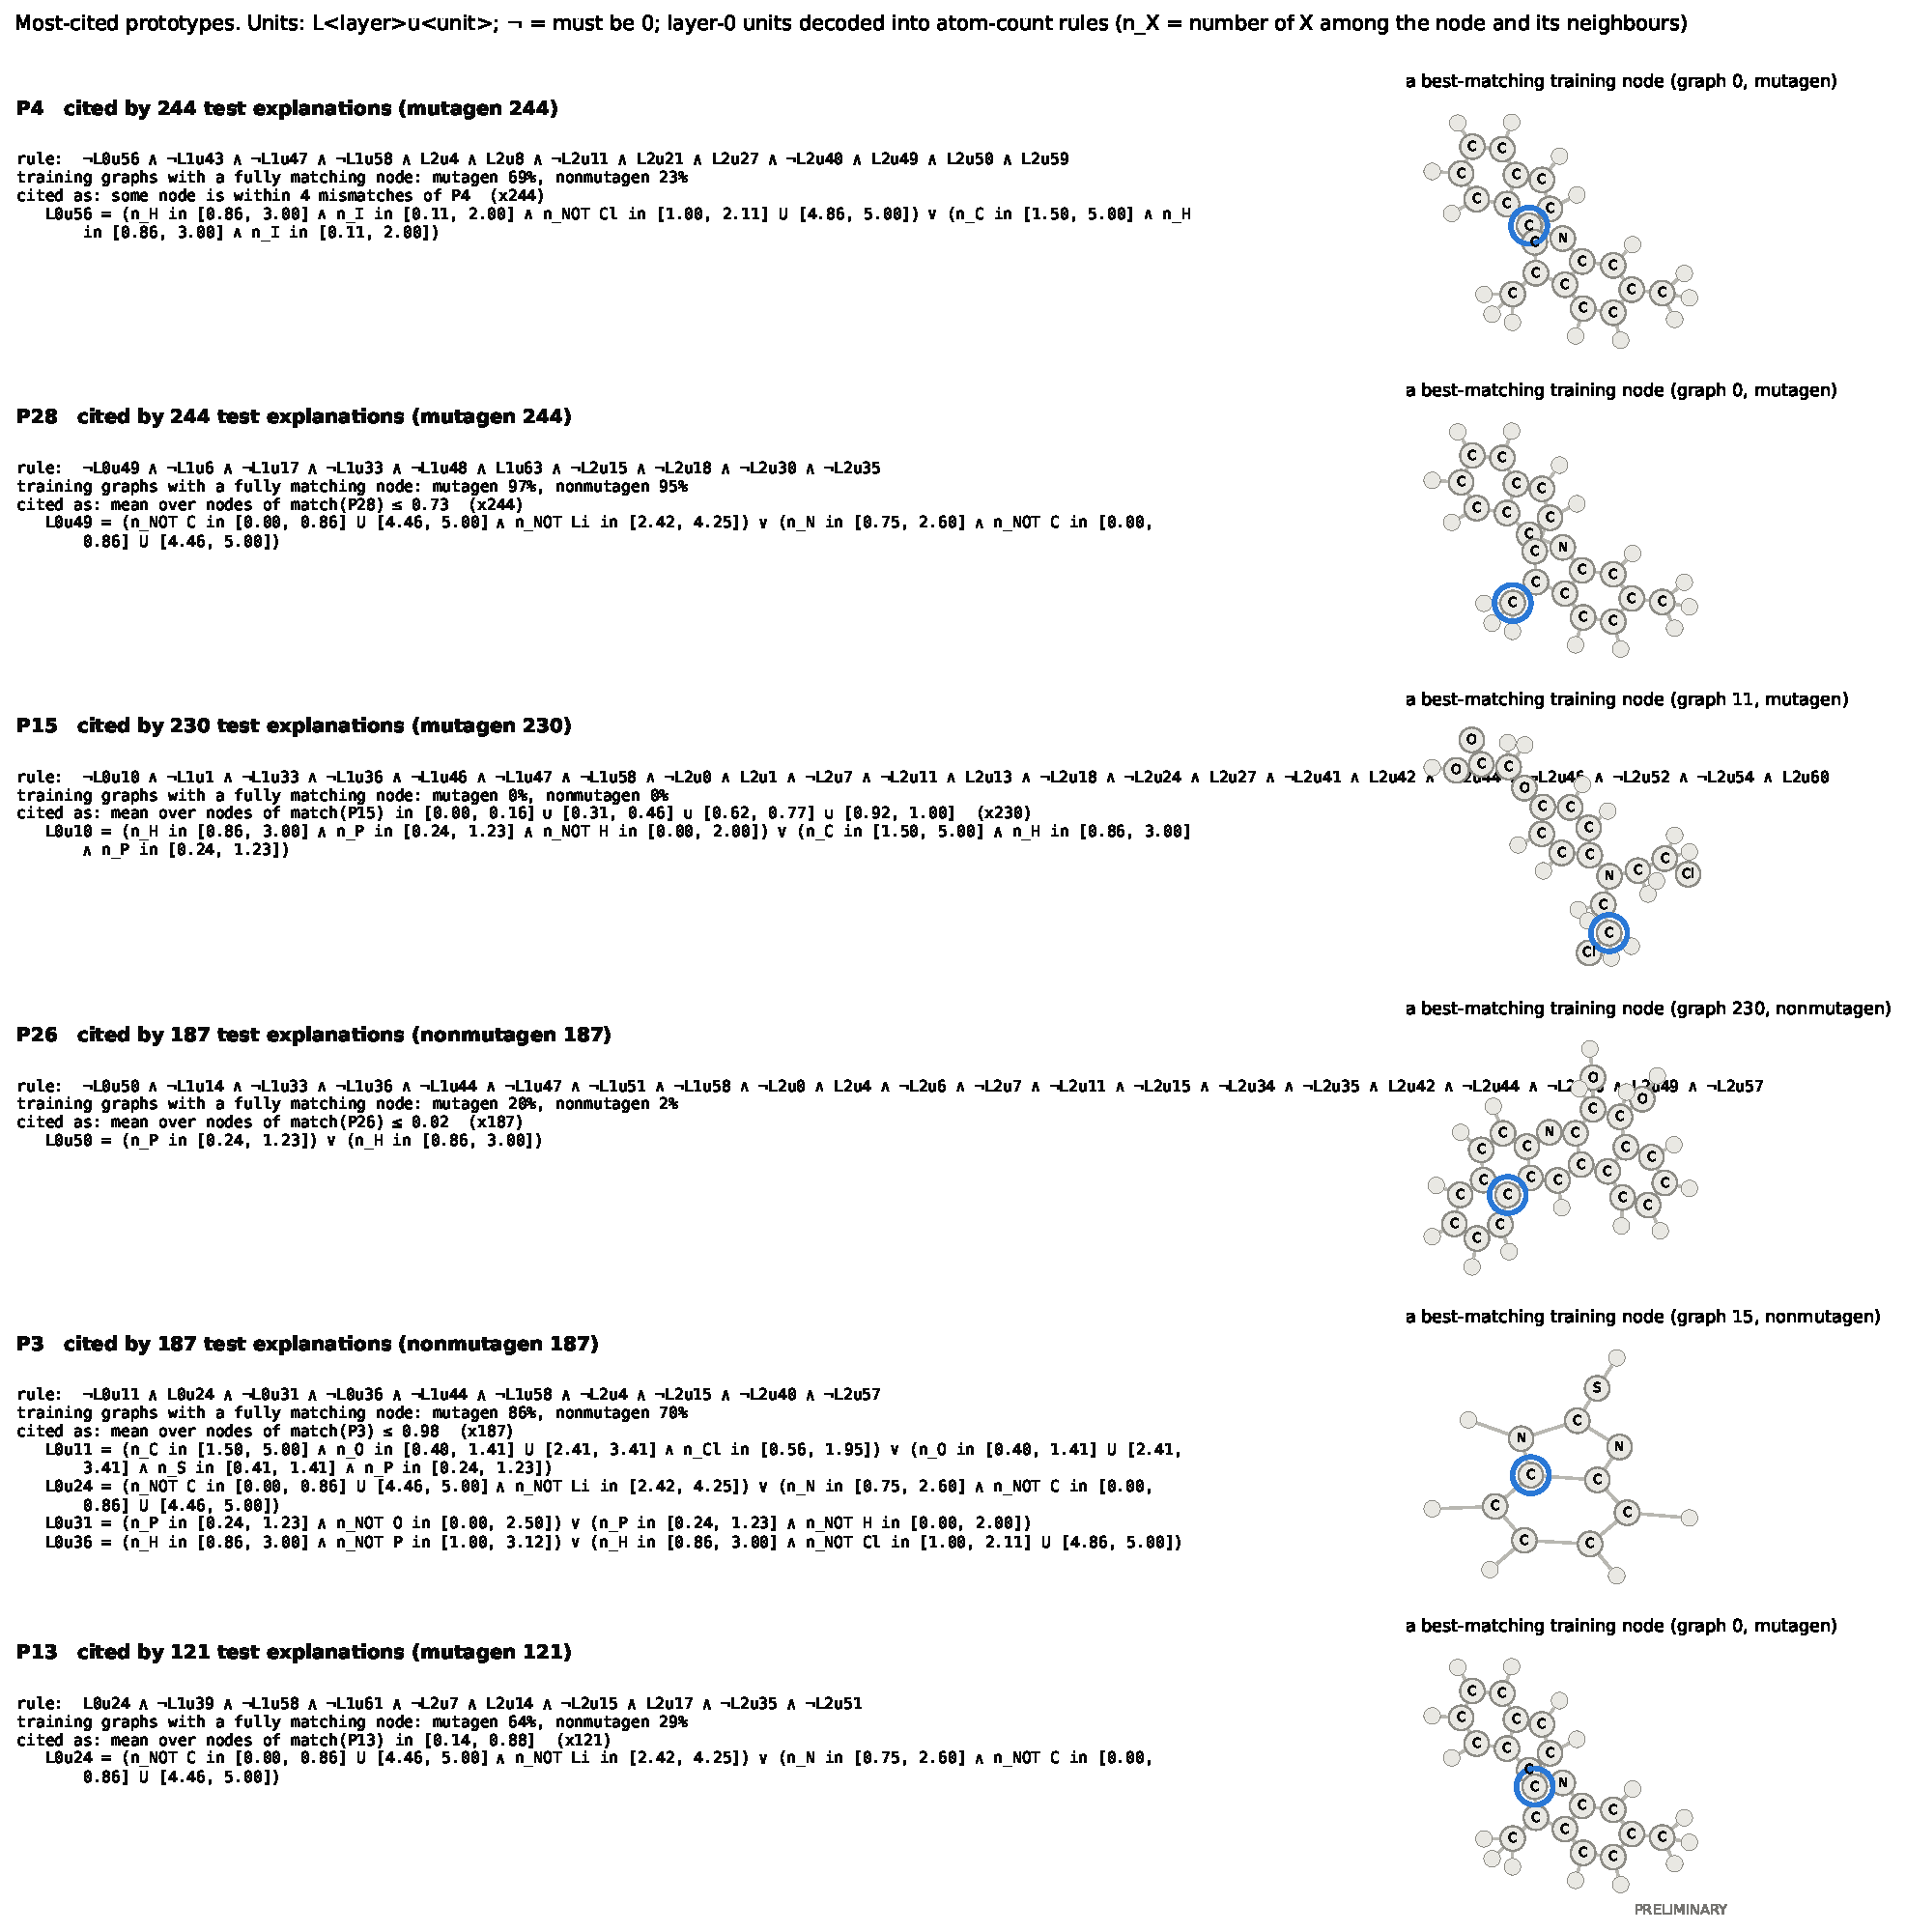
\includegraphics[width=\textwidth]{figures/fig_prototypes_Mutagenicity.pdf}%
  }{\fbox{\parbox[c][3cm]{0.95\textwidth}{\centering\todo{fig\_prototypes\_Mutagenicity.pdf}}}}\\[4pt]
  \IfFileExists{figures/fig_prototypes_BaMultiShapes.pdf}{%
    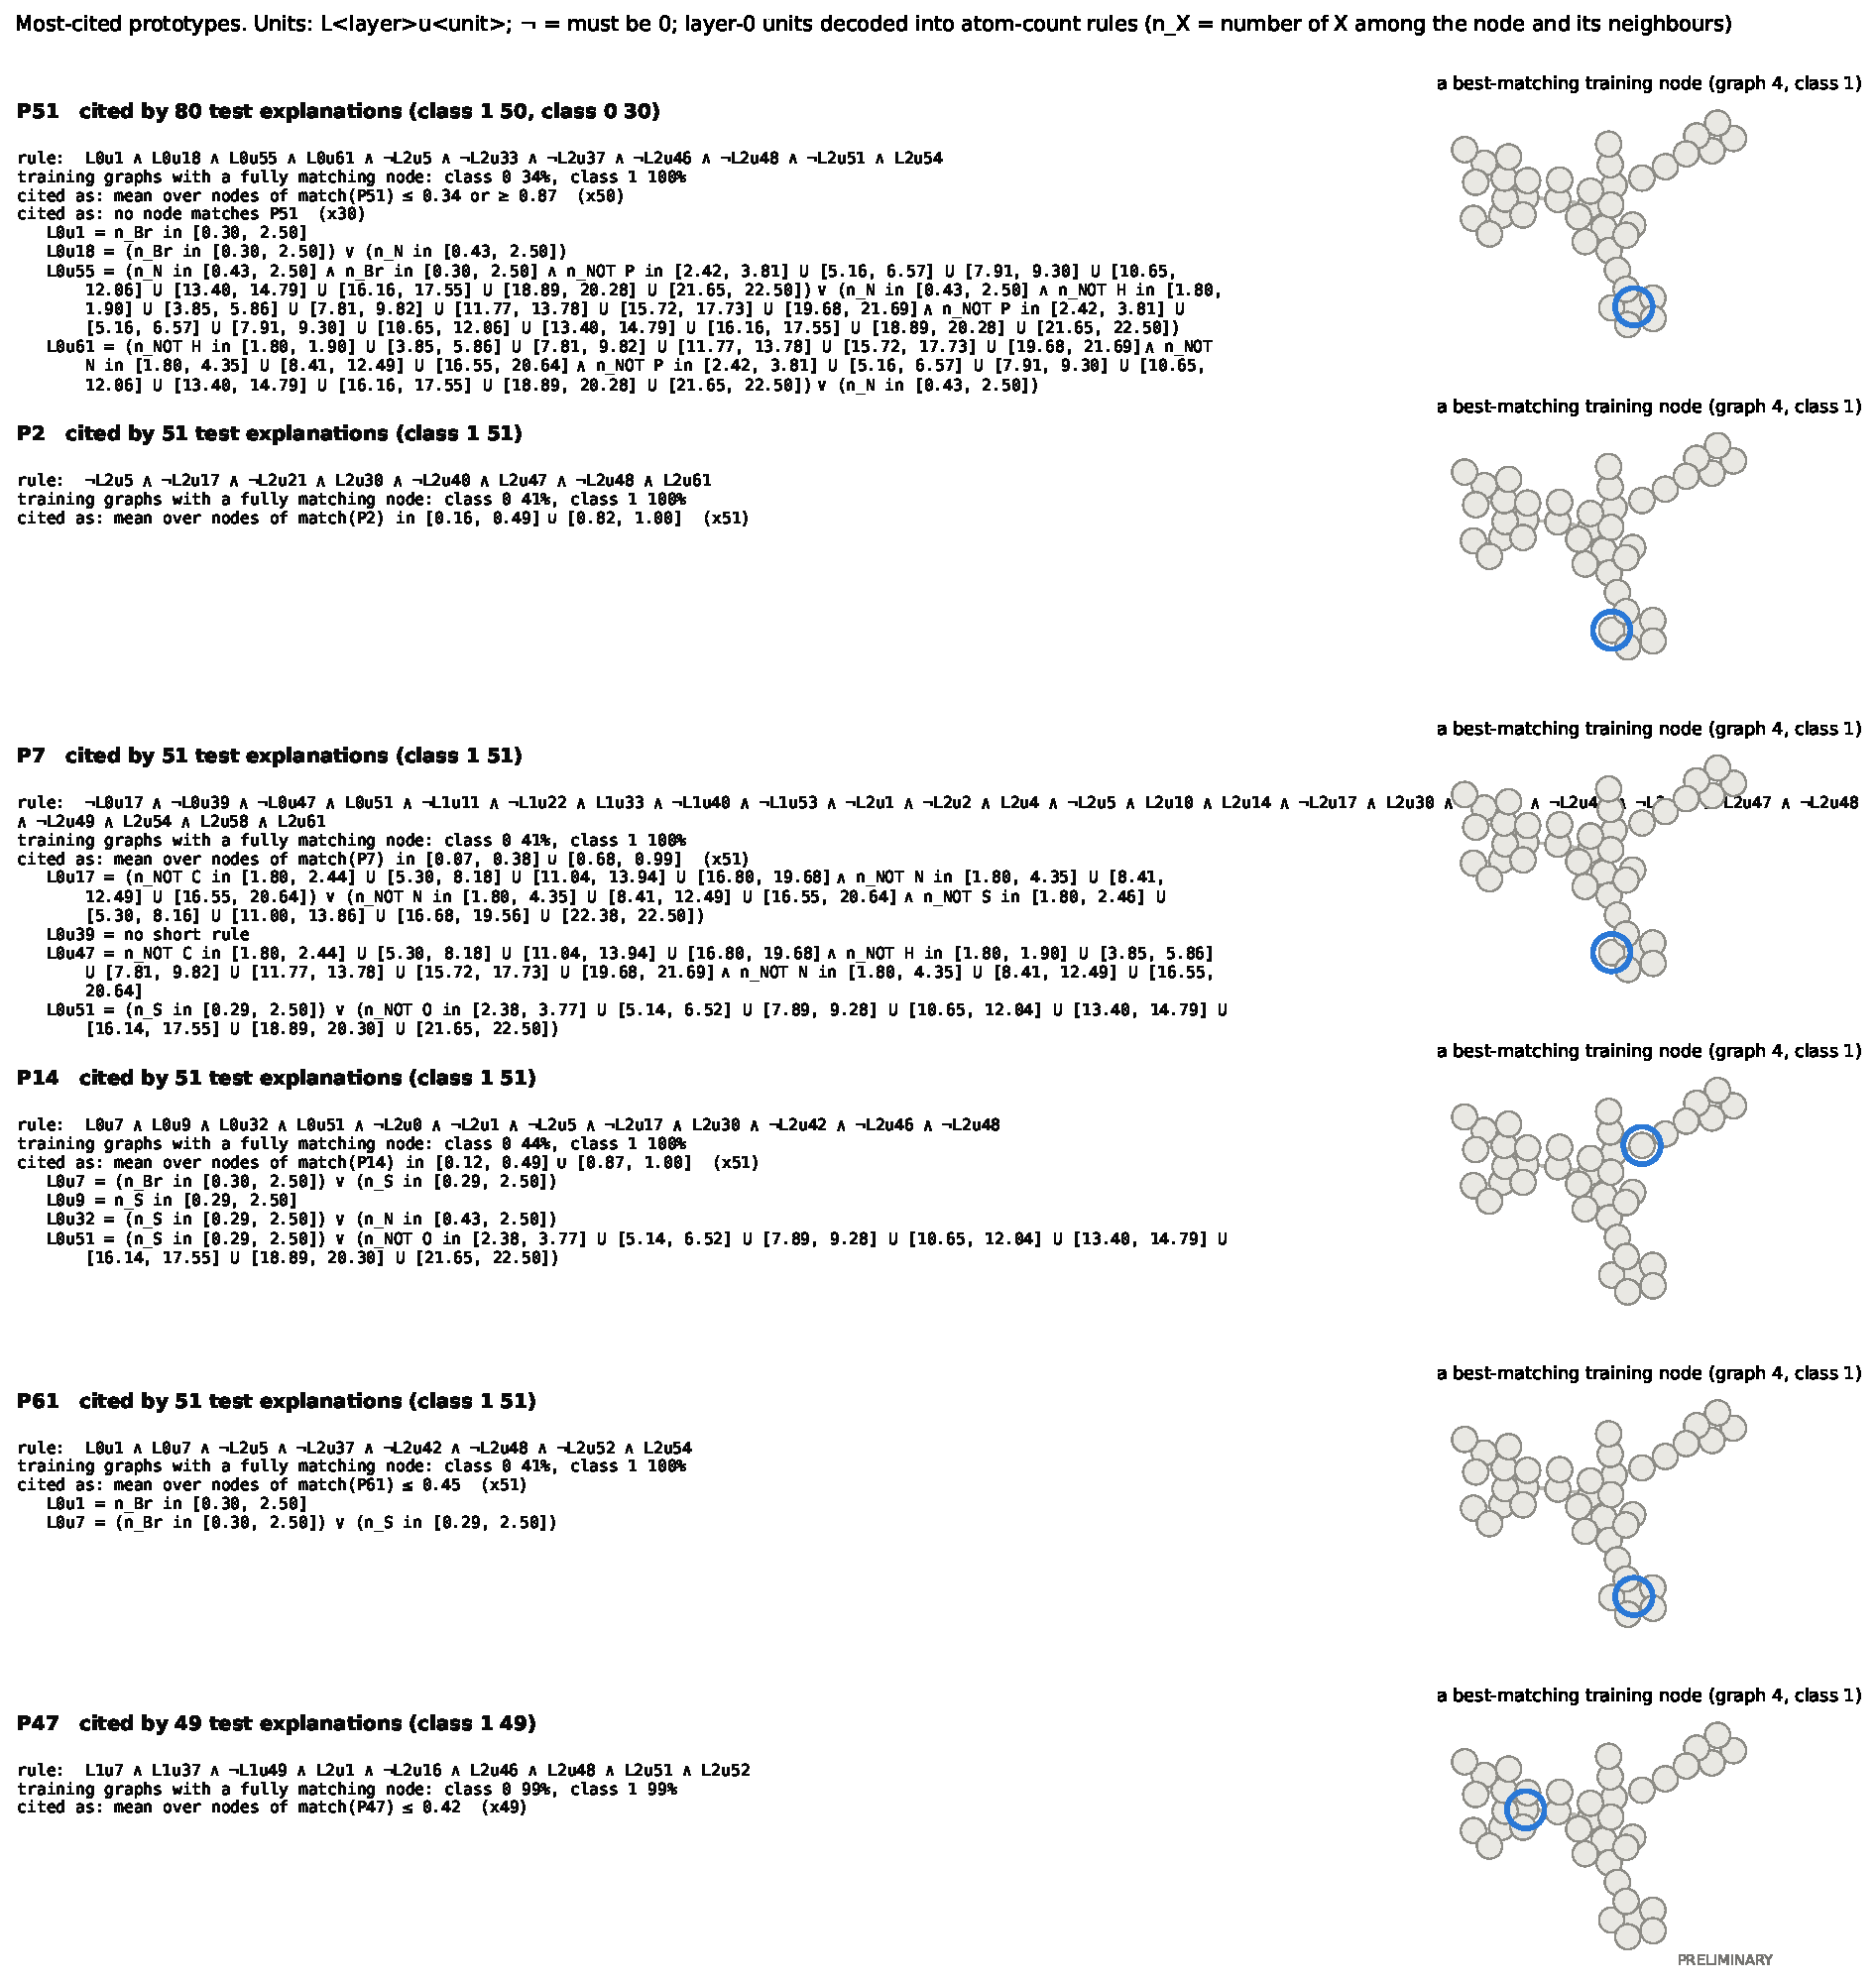
\includegraphics[width=\textwidth]{figures/fig_prototypes_BaMultiShapes.pdf}%
  }{\fbox{\parbox[c][3cm]{0.95\textwidth}{\centering\todo{fig\_prototypes\_BaMultiShapes.pdf}}}}\\[4pt]
  \caption{Prototypes of \oursqat{}. Each card shows the training node the
    prototype was projected on, the trunk conditions it cares about, and the best
    matching nodes of test graphs (highlighted; shaded: ground-truth region,
    NO$_2$/NH$_2$ on Mutagenicity, planted motifs on BAMultiShapes).}
  \label{fig:prototypes}
\end{figure*}

% =====================================================================================
% fig_explanation.tex: one prediction explained end to end (Q4; Notion E11).
%
% What the experiment tests: that the explanation of a single prediction can be read as
%   a short chain: class rule (head literals) -> prototypes it cites -> the matching nodes
%   in the input graph -> the trunk conditions on those nodes. Because the NMP+QAT
%   network computes exactly its rules, this chain IS the computation, not an
%   approximation of it.
% Plot: for one correctly predicted mutagen (and one non-mutagen, or one BAMultiShapes
%   graph): left, the graph with the nodes cited by the explanation highlighted; right,
%   the explanation tree (explorer/ "explanation tree"): class score = sum of true
%   literals >= threshold, each literal "graph has a node within t mismatches of Pk",
%   each Pk's cared bits as conditions. Constant literals greyed out / omitted
%   (evidence-only explanation).
% What it shows: what a user actually reads, and its length (e.g. 1-2 input-dependent
%   literals on Mutagenicity QAT fold 3).
% What it does not show: typical behaviour (one example; pick by a stated rule, e.g. a
%   random correctly classified test graph with seed, and add a failure case in the
%   appendix); readability of L1/L2 bits.
% Data: explorer export (python -m explorer export <run> --html) or SymbolicReader
%   (explorer/), final NMP+QAT fold of fig_prototypes.
% GENERATED BY: python plot_paper.py explanation   (sources: configs/paper_figures.yaml, code:
%   utils/paper_figures.py, branch feat/paper-figures). "preliminary: true" in the config
%   stamps PRELIMINARY on the figure; set it to false only when every source is final.
% STATUS: PRELIMINARY version drawn 2026-10-21 (qat_nmp, Mutagenicity test graph 5 of the representative fold). The head box lists constant literals too (use the evidence-only explanation), and the prototype box text overflows: needs a layout pass.
% TODO:
%   [ ] static export (SVG/PDF) of one explanation tree from explorer/ ->
%       paper/figures/fig_explanation.pdf.
% =====================================================================================
\begin{figure*}[t]
  \centering
  \IfFileExists{figures/fig_explanation.pdf}{%
    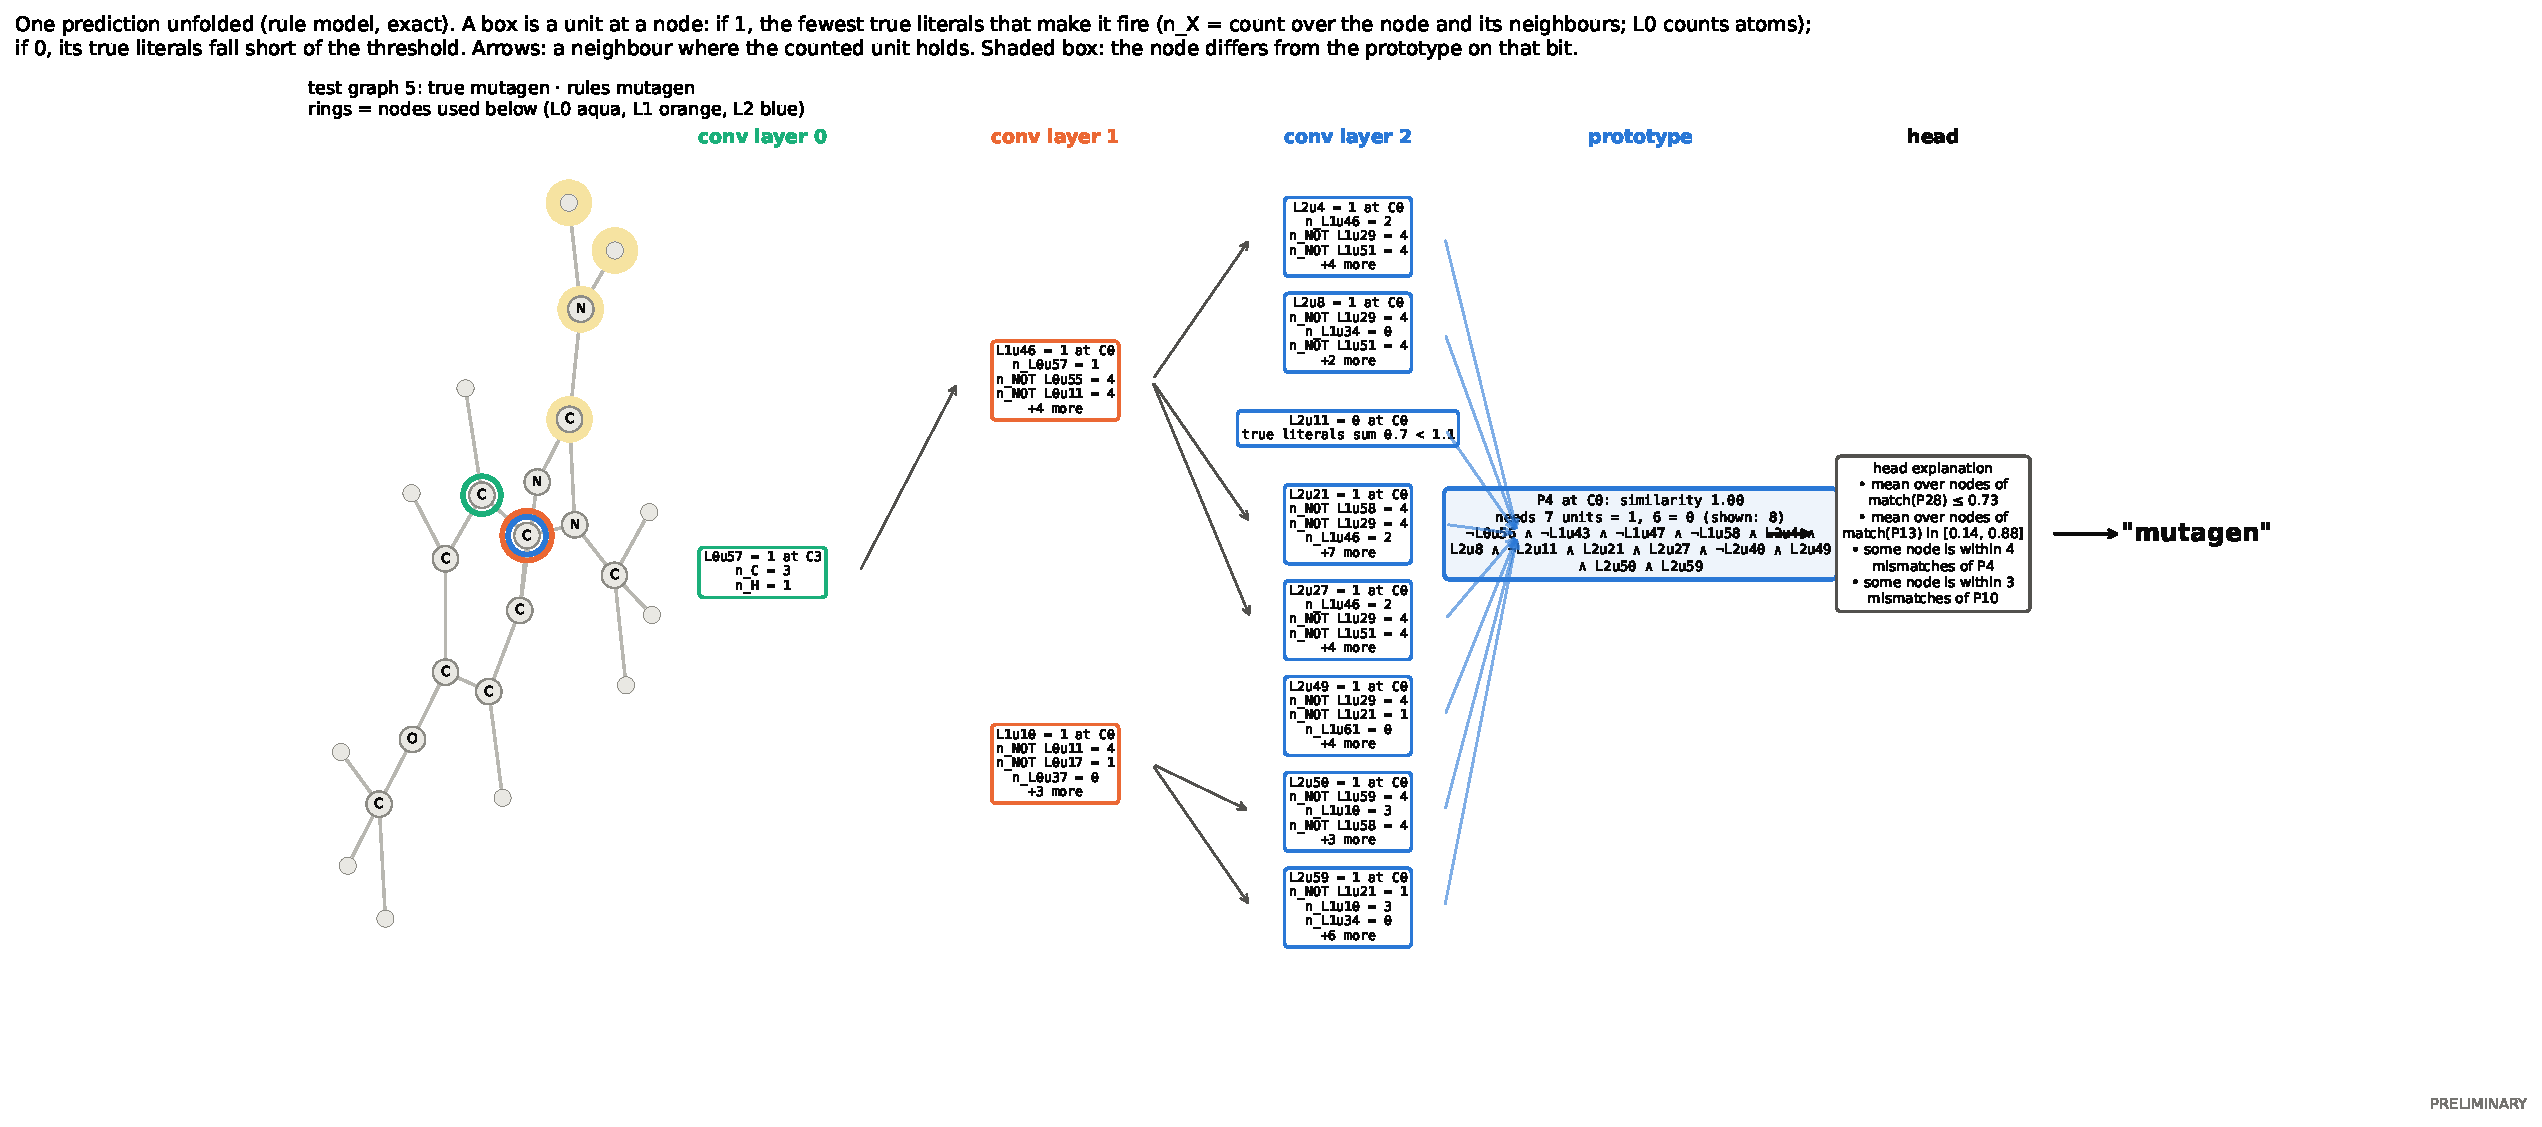
\includegraphics[width=\textwidth]{figures/fig_explanation.pdf}%
  }{\fbox{\parbox[c][5cm]{0.95\textwidth}{\centering\todo{fig\_explanation.pdf: one prediction explained}}}}
  \caption{Explanation of one test prediction on Mutagenicity. The class rule fires
    because the molecule contains nodes matching the cited prototypes (highlighted); each
    prototype is read as the trunk conditions it cares about. Since the network computes
    its rules exactly, this is the model's whole decision.}
  \label{fig:explanation}
\end{figure*}

\todo{paragraph}

% -------------------------------------------------------------------------------------
% Appendix material (move to the appendix file when it exists).
% =====================================================================================
% table_main_full.tex: appendix; every classification metric of the students (Q1, E1).
%
% Metrics: test accuracy, balanced accuracy, F1 of the minority class, ROC-AUC (%),
%   mean ± std over 10 folds (utils/evaluation.py). Of the network, not the rule model.
%
% STATUS: \prelim / \tbd everywhere; same sources and caveats as table_main.tex
%   (sum_ablation and sum_ablation_ctrl trained before the head-saturation fix of
%   2026-10-19; Mutagenicity graph / NMP from a hand-tuned set; ^3 = folds 0-2 only).
%   Rows were generated from results_final/<exp>/<dataset>/summary.csv (columns
%   test_{acc,balanced_acc,f1,auc}_{mean,std}).
%
% TODO:
%   [ ] fill from the final E1 experiment (table_main.tex TODO).
%   [ ] teacher rows: total_results.csv only has accuracy. Get the other metrics without
%       retraining, e.g. a CPU evaluation of the 10 best.pt per dataset written to a NEW
%       file (train_baseline.py --only_eval rewrites results.json / total_results.csv:
%       don't overwrite them).
%   [ ] competitors, same columns.
% =====================================================================================
\begin{table*}[p]
  \centering
  \caption{All test metrics of the self-explainable students (\%, mean $\pm$ std over 10
    folds): accuracy, balanced accuracy, F1 of the minority class and ROC-AUC.
    \prelim{Grey}: preliminary runs. $^3$: folds 0--2 only.}
  \label{tab:main_full}
  \small
  \begin{tabular}{llcccc}
    \toprule
    Dataset & Model & Acc. & Bal.\ acc. & F1 (minority) & ROC-AUC \\
    \midrule
    \multirow{5}{*}{MUTAG}   & \classic{} & \prelim{\ms{63.9}{19.0}} & \prelim{\ms{58.1}{16.4}} & \prelim{\ms{41.6}{25.8}} & \prelim{\ms{63.3}{25.9}} \\
                             & \classicnosum{} & \prelim{\ms{81.0}{9.6}} & \prelim{\ms{75.4}{15.1}} & \prelim{\ms{61.8}{29.6}} & \prelim{\ms{90.3}{8.6}} \\
                             & \oursgraph{} & \prelim{\ms{82.5}{13.0}} & \prelim{\ms{81.0}{13.3}} & \prelim{\ms{74.5}{18.6}} & \prelim{\ms{87.2}{9.7}} \\
                             & \oursnmp{} & \prelim{\ms{39.8}{13.9}} & \prelim{\ms{50.0}{0.0}} & \prelim{\ms{40.0}{21.2}} & \prelim{\ms{46.9}{9.7}} \\
                             & \oursqat{} & \tbd & \tbd & \tbd & \tbd \\
    \midrule
    \multirow{5}{*}{Mutagenicity} & \classic{} & \tbd & \tbd & \tbd & \tbd \\
                             & \classicnosum{} & \tbd & \tbd & \tbd & \tbd \\
                             & \oursgraph{} & \prelim{\ms{82.2}{1.4}} & \prelim{\ms{82.1}{1.5}} & \prelim{\ms{80.2}{1.8}} & \prelim{\ms{88.7}{1.5}} \\
                             & \oursnmp{} & \prelim{\ms{80.4}{2.1}} & \prelim{\ms{80.1}{2.1}} & \prelim{\ms{77.9}{2.5}} & \prelim{\ms{86.8}{1.6}} \\
                             & \oursqat{} & \prelim{\ms{76.6}{1.7}} & \prelim{\ms{76.2}{1.9}} & \prelim{\ms{73.4}{2.7}} & \prelim{\ms{82.4}{1.8}} \\
    \midrule
    \multirow{5}{*}{AIDS}    & \classic{} & \tbd & \tbd & \tbd & \tbd \\
                             & \classicnosum{} & \tbd & \tbd & \tbd & \tbd \\
                             & \oursgraph{} & \tbd & \tbd & \tbd & \tbd \\
                             & \oursnmp{} & \tbd & \tbd & \tbd & \tbd \\
                             & \oursqat{} & \tbd & \tbd & \tbd & \tbd \\
    \midrule
    \multirow{5}{*}{BBBP}    & \classic{} & \tbd & \tbd & \tbd & \tbd \\
                             & \classicnosum{} & \tbd & \tbd & \tbd & \tbd \\
                             & \oursgraph{} & \tbd & \tbd & \tbd & \tbd \\
                             & \oursnmp{} & \tbd & \tbd & \tbd & \tbd \\
                             & \oursqat{} & \tbd & \tbd & \tbd & \tbd \\
    \midrule
    \multirow{5}{*}{NCI1}    & \classic{} & \tbd & \tbd & \tbd & \tbd \\
                             & \classicnosum{} & \tbd & \tbd & \tbd & \tbd \\
                             & \oursgraph{} & \tbd & \tbd & \tbd & \tbd \\
                             & \oursnmp{} & \tbd & \tbd & \tbd & \tbd \\
                             & \oursqat{} & \tbd & \tbd & \tbd & \tbd \\
    \midrule
    \multirow{5}{*}{PROTEINS} & \classic{} & \prelim{\ms{73.7}{4.4}} & \prelim{\ms{72.0}{4.1}} & \prelim{\ms{66.1}{5.1}} & \prelim{\ms{79.9}{5.2}} \\
                             & \classicnosum{} & \prelim{\ms{69.4}{8.6}} & \prelim{\ms{65.1}{10.8}} & \prelim{\ms{47.9}{28.1}} & \prelim{\ms{76.4}{7.8}} \\
                             & \oursgraph{} & \prelim{\ms{75.1}{4.9}} & \prelim{\ms{73.4}{5.4}} & \prelim{\ms{67.4}{7.6}} & \prelim{\ms{79.5}{5.5}} \\
                             & \oursnmp{} & \prelim{\ms{74.2}{3.7}} & \prelim{\ms{72.7}{3.7}} & \prelim{\ms{67.0}{4.7}} & \prelim{\ms{77.3}{3.8}} \\
                             & \oursqat{} & \prelim{\ms{75.3}{4.0}$^3$} & \prelim{\ms{72.7}{4.9}$^3$} & \prelim{\ms{65.5}{7.8}$^3$} & \prelim{\ms{76.8}{7.4}$^3$} \\
    \midrule
    \multirow{5}{*}{BA2Motifs} & \classic{} & \tbd & \tbd & \tbd & \tbd \\
                             & \classicnosum{} & \tbd & \tbd & \tbd & \tbd \\
                             & \oursgraph{} & \tbd & \tbd & \tbd & \tbd \\
                             & \oursnmp{} & \tbd & \tbd & \tbd & \tbd \\
                             & \oursqat{} & \tbd & \tbd & \tbd & \tbd \\
    \midrule
    \multirow{5}{*}{BAMultiShapes} & \classic{} & \prelim{\ms{99.1}{0.9}} & \prelim{\ms{99.1}{0.9}} & \prelim{\ms{99.1}{0.9}} & \prelim{\ms{99.9}{0.2}} \\
                             & \classicnosum{} & \prelim{\ms{95.9}{3.0}} & \prelim{\ms{95.9}{3.0}} & \prelim{\ms{95.7}{3.2}} & \prelim{\ms{98.2}{2.1}} \\
                             & \oursgraph{} & \prelim{\ms{99.3}{0.8}} & \prelim{\ms{99.3}{0.8}} & \prelim{\ms{99.3}{0.8}} & \prelim{\ms{100.0}{0.0}} \\
                             & \oursnmp{} & \prelim{\ms{98.0}{2.4}} & \prelim{\ms{98.0}{2.4}} & \prelim{\ms{97.9}{2.5}} & \prelim{\ms{99.6}{0.9}} \\
                             & \oursqat{} & \prelim{\ms{98.7}{0.6}$^3$} & \prelim{\ms{98.7}{0.6}$^3$} & \prelim{\ms{98.6}{0.6}$^3$} & \prelim{\ms{99.3}{1.2}$^3$} \\

    \bottomrule
  \end{tabular}
\end{table*}

% =====================================================================================
% table_sensitivity.tex: appendix; sensitivity to trunk width and to the vocabulary
%   penalty (Notion E9, E10; P2).
%
% Questions:
%   E9  does a narrower trunk (width 32 instead of 64) trade accuracy for fidelity and
%       shorter rules? (earlier random-split result: width 32 raised classic fidelity to
%       0.84 but lowered NO2/NH2 precision)
%   E10 effect of vocab_reg (penalty on the number of distinct trunk units the prototypes
%       read) on explanation size and accuracy (0.1 was best on random splits).
% Protocol (to write): best E1 NMP set, change one factor, 10 folds. Width 32 needs its
%   own k-fold teachers (teacher hidden_dim 32: train_baseline.py, new teacher config;
%   ~10 teachers per dataset). vocab_reg in {0, 0.01, 0.1, 0.3}.
% Datasets: Mutagenicity (GT) + PROTEINS.
% What it should show: whether the paper's defaults are a sweet spot or arbitrary.
% What it will not show: joint effects (one factor at a time).
%
% STATUS: NOT RUN. Code: experiment YAML with params_from + per-row fixed overrides
%   (check utils/experiment.py supports a fixed override per model entry, else add model
%   entries). Teachers of width 32 = new teacher config.
% TODO:
%   [ ] E10 first (no new teachers), E9 if time.
% =====================================================================================
\begin{table}[t]
  \centering
  \caption{Sensitivity of \nmp{} to the trunk width and to the vocabulary penalty (test,
    10 folds, \%). Bits: explanation size; GT prec.: Mutagenicity NO$_2$/NH$_2$.}
  \label{tab:sensitivity}
  \small
  \setlength{\tabcolsep}{3.5pt}
  \begin{tabular}{llccccc}
    \toprule
    & & \multicolumn{3}{c}{Mutagenicity} & \multicolumn{2}{c}{PROTEINS} \\
    \cmidrule(lr){3-5}\cmidrule(lr){6-7}
    Factor & Value & Rule acc. & Bits & GT prec. & Rule acc. & Bits \\
    \midrule
    \multirow{2}{*}{Trunk width}
      & 32 & \tbd & \tbd & \tbd & \tbd & \tbd \\
      & 64 & \tbd & \tbd & \tbd & \tbd & \tbd \\
    \midrule
    \multirow{4}{*}{Vocabulary penalty}
      & 0    & \tbd & \tbd & \tbd & \tbd & \tbd \\
      & 0.01 & \tbd & \tbd & \tbd & \tbd & \tbd \\
      & 0.1  & \tbd & \tbd & \tbd & \tbd & \tbd \\
      & 0.3  & \tbd & \tbd & \tbd & \tbd & \tbd \\
    \bottomrule
  \end{tabular}
\end{table}


\InputIfFileExists{5_conclusion.tex}{}{}

\IfFileExists{references.bib}{%
  \bibliographystyle{plain}
  \bibliography{references}
}{}

\appendix
\section{Hyper-parameter search spaces}
\label{app:hps}
\todo{table of configs/search\_spaces.yaml and the fixed arguments of configs/models.yaml}

\end{document}
